%%%%%%%%%%%%%%%%%%%%%%% file template.tex %%%%%%%%%%%%%%%%%%%%%%%%%
%
% This is a general template file for the LaTeX package SVJour3
% for Springer journals.          Springer Heidelberg 2010/09/16
%
% Copy it to a new file with a new name and use it as the basis
% for your article. Delete % signs as needed.
%
% This template includes a few options for different layouts and
% content for various journals. Please consult a previous issue of
% your journal as needed.
%
%%%%%%%%%%%%%%%%%%%%%%%%%%%%%%%%%%%%%%%%%%%%%%%%%%%%%%%%%%%%%%%%%%%
%
% \RequirePackage{fix-cm}
%
%\documentclass{svjour3}                     % onecolumn (standard format)
% \documentclass[smallcondensed]{svjour3}     % onecolumn (ditto)
%\documentclass[smallextended]{svjour3}       % onecolumn (second format)
%\documentclass[twocolumn]{svjour3}          % twocolumn
%
% \smartqed  % flush right qed marks, e.g. at end of proof
%

%
% \usepackage{mathptmx}      % use Times fonts if available on your TeX system
%
% insert here the call for the packages your document requires
%\usepackage{latexsym}
% etc.
%
% please place your own definitions here and don't use \def but
% \newcommand{}{}
%
% Insert the name of "your journal" with
% \journalname{myjournal}
%


%personal adding

% \usepackage{program}
% \savesymbol{AND}
% \savesymbol{OR}
% \savesymbol{NOT}
% \savesymbol{TO}
% \savesymbol{COMMENT}
% \savesymbol{BODY}
% \savesymbol{IF}
% \savesymbol{ELSE}
% \savesymbol{ELSIF}
% \savesymbol{FOR}
% \savesymbol{WHILE}

% \newcommand{\Rset}{\mathbb{R}}
% \newcommand{\IRset}{\mathbb{IR}}



% correct bad hyphenation here
\hyphenation{op-tical net-works semi-conduc-tor}

\graphicspath{{part_1/figures}{part_1/figures/}}


In this chapter, we present practical ways to compute the Post and Tube operators 
when sets are represented with boxes or balls.
We first give some results for linear systems. We then present approaches
relying on Runge-Kutta schemes, allowing to compute accurately images of box sets 
for nonlinear ODEs. We then introduce some hypotheses to use a simple Euler scheme,
associated to a new error bound, permitting to compute the Post and Tube operators
for balls in a very fast way, even though the accuracy can fall down in some cases. 

\section{Zonotopes and linear systems}
\label{chap:1.1}

Let us first introduce {\em zonotopes}, a type of symmetrical polytopes, allowing to represent 
efficiently boxes of $\R^n$, and for which there exist multiple ways to compute
their images by linear or nonlinear transformations.

\begin{definition}

  A {\em zonotope} is a set:
  $$ Z = \{ x \in \R^n : x = c + \sum_{i= 1}^p \beta^{(i)} g^{(i)}, \ -1 \leq \beta^{(i)} \leq 1 \}$$
with $c$, $g^{(1)}$,\dots,$g^{(p)} \in \R^n$. 
 \label{def:zonotope}
\end{definition}

The vectors $g^{(1)}$,$\dots$,$g^{(p)}$ are referred to as the {\em generators} and $c$ 
as the center of a zonotope. A zonotope is thus a symmetric polytope in dimension $n$. 
It is convenient to represent the set of generators as an $n \times p$ matrix $G$, of columns
$g^{(1)}$,$\dots$,$g^{(p)}$. The notation is $< c,G>$. 

Given a zonotope $< c , G>$, the transformation of $z$ via an affine function 
$ x \longrightarrow C x + d$ is a zonotope of the form $< Cc + d, CG >$.
More information and properties on zonotopes can be found in \cite{???}. 
Besides, 
being given a linear switched system satisfying 
$$ \dot x = A_j x + b_j,$$ and an initial condition $x_0 \in \R^n$ at time $t = 0$,
if mode $j \in U$ is applied on $[ 0 , \tau]$, then 
the solution at time $t = \tau$ is given by
$$ \phi (t;0,x_0,j) = e^{A_j \tau} x_0 +   \int_0^\tau e^{A_j (t-s)} b_j ds. $$
In the case where $A_j$ is invertible, we furthermore have
$$ \phi (t;0,x_0,j) = e^{A_j \tau} x_0 +   ( e^{A_j \tau} - I_n ) A_j ^{-1} b_j$$
where $I_n$ is the identity matrix of size $n$.
In both cases we have an affine transformation.   
One can thus compute exactly the image of a set using zonotopes.
Take an initial set given at time $t=0$ as a zonotope $Z = <c,G>$, 
its image (successor set) at time $t = \tau$ is (for $A_j$ invertible) 
$Z' = Post_j(Z) =  < e^{A_j \tau} c +   ( e^{A_j \tau} - I_n ) A_j ^{-1} b_j, e^{A_j \tau} G>$.
This formula can be iterated to obtain the successor set at time $t = k \tau$ of $Z$
via a pattern $\pi = (j_1, \dots, j_k)$ for $k \in \N_{>0}$:
$ Post_\pi (Z) = Post_{j_k} (Post_{j_{k-1}} ( \dots Post_{j_1} (Z)))$.

While computing the Tube operator is still a difficult task for linear systems,
computing the Post operator in this way, 
associated to Algorithm \ref{algo:decomposition} and \ref{algo:findpattern2} (without the 
safety property relying on the Tube), we can compute 
controllers permitting to return infinitely often in a set $R$ thanks to
Theorem \ref{th:R-procedure}. 
This approach can also be used to ensure discrete-time properties, i.e., 
which are not ensured between switchings but at discrete times $\tau$, $2\tau$...
This approach is efficient and useful in practice, all the more so as
the Post operator is computed exactly.








\section{Validated simulation and state-space bisection}



In general, the exact solution of differential equations cannot be
obtained, and a numerical integration scheme is used to approximate
the state of the system.  With the objective of computing a guaranteed
control, we base our approach on validated simulation (also called
``reachability analysis''). The \emph{guaranteed} or \emph{validated}
solution of ODEs using interval arithmetic is mainly built over two
kinds of methods based on: i) Taylor
series~\cite{Moore66,Nedialkov,LiSt07,Dzetkulic:2015fk} ii)
Runge-Kutta schemes~\cite{BM06,Gajda:2008fk,BCD13,report}. The former
is the oldest method used in interval analysis community because the
expression of the remainder of Taylor series is simple to obtain.
Nevertheless, the family of Runge-Kutta methods is very important in
the field of numerical analysis.  Indeed, Runge-Kutta methods have
several interesting stability properties which make them suitable for
an important class of problems. Recent work~\cite{dynibex} implements
Runge-Kutta based methods which prove their efficiency at low orders
and for short simulations (fixed by sampling period of controller).

In the methods of symbolic analysis and control of hybrid systems, the
way of representing sets of state values and computing reachable sets
for systems defined by autonomous ordinary differential equations
(ODEs), is fundamental (see for
example~\cite{girard2005reachability,althoff2013reachability}). Many
tools using, \textit{e.g.}, linearization or hybridization of these
dynamics are now available (\textit{e.g.},
SpaceEx~\cite{frehse2011spaceex}, Flow*~\cite{chen2013flow},
iSAT-ODE~\cite{eggers2008sat}).  An interesting approach appeared
recently, based on the propagation of reachable sets using guaranteed
Runge-Kutta methods with adaptive step-size control (see
\cite{BCD13,immler2015verified}).

An originality of our work is to use such guaranteed integration
methods in the framework of switched systems. This notion of guarantee
of the results is very interesting, because it allows applications in
critical domains, such as aeronautical, military and medical ones.
Other symbolic approaches for control synthesis of switched systems
include the construction of a discrete abstraction of the original
system on a grid of the state space. This can be done by computing
symbolic models that are approximately bisimilar
\cite{girard2010approximately} or approximately alternatingly similar
\cite{zamani2012symbolic} to the original system.  Another recent
symbolic approach relies on feedback refinement relations
\cite{reissig2015feedback}. We compare our work with the last two
approaches, which are the closest related methods since the associated
tools (respectively PESSOA~\cite{Mazo2010} and SCOTS~\cite{SCOTS}) are
used to perform control synthesis on switched systems without any
stability assumptions, such as the present method.


% The paper is divided as follows. In Section~\ref{sec:switched}, we
% introduce some preliminaries on switched systems and some notation
% used in the following. In Section~\ref{sec:simulation}, the guaranteed
% integration of nonlinear ODEs is presented. In
% Section~\ref{sec:minimator}, we present the main algorithm of
% state-space bisection used for control synthesis.  In
% Section~\ref{sec:experimentations}, the whole approach is tested on
% four examples of the literature.  We give some performance tests and
% compare our approach with the state-of-the-art tools in
% Section~\ref{sec:comparison}.  We conclude in
% Section~\ref{sec:conclu}.



\subsection{Validated simulation}
\label{sec:simulation}

In this subsection, we describe our approach for validated simulation
based on Runge-Kutta methods~\cite{BCD13,report}. The goal being
obviously to obtain a solution of the differential equations
describing the modes of the nonlinear switched systems. Before
presenting the method, we introduce some definitions.


In the following, we will often use the notation $\lbrack x \rbrack
\in \IRset$ (the set of intervals with real bounds) where
\begin{displaymath}
  \lbrack x \rbrack =
  \lbrack\underline{x}, \overline{x}\rbrack=
  \{ x \in \Rset \mid \underline{x} \leqslant x \leqslant \overline{x} \}
\end{displaymath}
denotes an interval.  By an abuse of notation $[x]$ will also denote a
vector of intervals, \emph{i.e.}, a Cartesian product of intervals,
a.k.a. a \emph{box}. In the following, the sets $R$, $S$ and $B$ are
given under the form of boxes. With interval values, it comes an
associated interval arithmetic.

\textit{Interval arithmetic} extends to $\IRset$ elementary functions
over $\Rset$. For instance, the interval sum, \textit{i.e.},
$[x_1]+[x_2]=[\underline{x_1}+\underline{x_2},
\overline{x_1}+\overline{x_2}]$, encloses the image of the sum
function over its arguments. The enclosing property basically defines
what is called an {\it interval extension} or an \emph{inclusion
  function}.

\begin{definition}[Inclusion function]
  Consider a function $f: \Rset^n \rightarrow \Rset^m$, then $[f]\!:\!
  \IRset^n \rightarrow \IRset^m$ is said to be an extension of $f$ to
  intervals if
  \begin{displaymath}
    \forall [{x}] \in \IRset^n, \quad [f]([{x}])
    \supseteq \{f({x}), {x} \in [{x}]\}\enspace.
  \end{displaymath}
\end{definition}

It is possible to define inclusion functions for all elementary
functions such as $\times$, $\div$, $\sin$, $\cos$, $\exp$, and so
on. The \emph{natural} inclusion function is the simplest to obtain:
all occurrences of the real variables are replaced by their interval
counterpart and all arithmetic operations are evaluated using interval
arithmetic. More sophisticated inclusion functions such as the
centered form, or the Taylor inclusion function may also be used
(see~\cite{JKDW01} for more details).

We now introduce the Initial Value Problem, which is one of main
ingredient of our approach.

\begin{definition}[Initial Value Problem (IVP)]
  Consider an ODE with a given initial condition
  \begin{equation}
    \label{eq:ivp}
    \dot{x}(t) = f(t, x(t), d(t))\quad\text{with}
    \quad x(0) \in X_0, \ d(t) \in \lbrack d \rbrack,
  \end{equation}
  with $f:\Rset^+\times\Rset^n\times \Rset^m\rightarrow\Rset^n$
  assumed to be continuous in $t$ and $d$ and globally Lipschitz in
  $x$. We assume that parameters $d$ are bounded (used to represent a
  perturbation, a modeling error, an uncertainty on
  measurement,~\dots).  An \emph{IVP} consists in finding a function
  $x(t)$ described by Equation~\eqref{eq:ivp} for all 
  $d(t)$ lying in $\lbrack d \rbrack$ and for all the initial
  conditions in $X_0$.
\end{definition}



A numerical integration method computes a sequence of values $(t_n,
x_n)$ approximating the solution $x(t;x_0)$ of the IVP defined in
Equation~\eqref{eq:ivp} such that $x_n \approx x(t_n;x_{n-1})$. The
simplest method is Euler's method in which $t_{n+1}=t_n+h$ for some
step-size $h$ and $x_{n+1}=x_n+h\times f(t_n,x_n, d)$; so the
derivative of $x$ at time $t_n$, $f(t_n,x_n, d)$, is used as an
approximation of the derivative on the whole time interval to perform
a linear interpolation. This method is very simple and fast, but
requires small step-sizes. More advanced methods, coming from the
Runge-Kutta family, use a few intermediate computations to improve the
approximation of the derivative. The general form of an explicit
$s$-stage Runge-Kutta formula, that is using $s$ evaluations of $f$,
is
\begin{equation}
  \begin{aligned}
    x_{n+1}  = x_n + h \sum_{i=1}^s b_i k_i\enspace, \\
    k_1  = f\big(t_n,\, x_n, d\big)\enspace,\\
    k_i  = f \Big(t_n + c_i h,\, x_n + h \sum_{j=1}^{i-1} a_{ij}k_j, d\Big)
    , \ i = 2,3,\dots,s\enspace.
    \label{eq:ki}
  \end{aligned}
\end{equation}
The coefficients $c_i$, $a_{ij}$ and $b_i$ fully characterize the
method. To make Runge-Kutta validated, the challenging question is how
to compute guaranteed bounds of the distance between the true solution
and the numerical solution, defined by $x(t_n;x_{n-1}) - x_n$. This
distance is associated to the \emph{local truncation error} (LTE) of
the numerical method.

To bound the LTE, we rely on \textit{order condition}~\cite{HNW93}
respected by all Runge-Kutta methods. This condition states that a
method of this family is of order $p$ iff the $p+1$ first coefficients
of the Taylor expansion of the solution and the Taylor expansion of
the numerical methods are equal. In consequence, LTE is proportional
to the Lagrange remainders of Taylor expansions.  Formally, LTE is
defined by (see~\cite{BCD13}):
\begin{multline}
  \label{eq:truncation-error}
  x(t_n;x_{n-1}) - x_n = \\
  \hspace{5mm}\frac{h^{p+1}}{(p+1)!} \left( f^{(p)}\left(\xi,x(\xi; x_{n-1}), d
    \right) - \frac{d^{p+1}\phi}{dt^{p+1}}(\eta) \right)
  \\
  \xi\in]t_n, t_{n+1}[ \text{ and } \eta\in]t_n, t_{n+1}[\enspace.
\end{multline}
The function $f^{(n)}$ stands for the $n$-th derivative of function
$f$ w.r.t. time $t$ that is $\frac{d^n f}{dt^n}$ and $h=t_{n+1}-t_n$
is the step-size.  The function $\phi:\Rset\to\Rset^n$ is defined by
$\phi(t)= x_n + h \sum_{i=1}^s b_i k_i(t)$ where $k_i(t)$ are defined
as Equation~\eqref{eq:ki}.

The challenge to make Runge-Kutta integration schemes safe w.r.t. the
true solution of IVP is then to compute a bound of the result of
Equation~\eqref{eq:truncation-error}. In other words, we do have to
bound the value of $f^{(p)}\left(\xi, x(\xi;x_{n-1}), d\right)$ and
the value of $\frac{d^{p+1}\phi}{dt^{p+1}}(\eta)$ with numerical
guarantee. The latter expression is straightforward to bound because
the function $\phi$ only depends on the value of the step-size $h$,
and so does its $(p+1)$-th derivative. The bound is then obtained
using the affine arithmetic~\cite{AffineA97,alexandre2016validated}.

However, the expression $f^{(p)}\left(\xi, x(\xi;x_{n-1}), d\right)$
is not so easy to bound as it requires to evaluate $f$ for a
particular value of the IVP solution $x(\xi;x_{n-1})$ at an unknown
time $\xi \in ]t_n, t_{n+1}[$. The solution used is the same as the
one found in~\cite{Nedialkov,BM06} and it requires to bound the
solution of IVP on the interval $[t_n, t_{n+1}]$. This bound is
usually computed using the Banach's fixpoint theorem applied with the
Picard-Lindel\"of operator, see~\cite{Nedialkov}. This operator is
used to compute an enclosure of the solution $[\tilde{x}]$ of IVP over
a time interval $[t_n, t_{n+1}]$, that is for all $t \in [t_n,
t_{n+1}]$, $x(t; x_{n-1}) \in [\tilde{x}]$. We can hence bound
$f^{(p)}$ substituting $x(\xi;x_{n-1})$ by $[\tilde{x}]$. This general
approach used to solve IVPs in a validated way is called Lohner two
step approach~\cite{Lohner87}.

\begin{figure}[t]
 \centering
 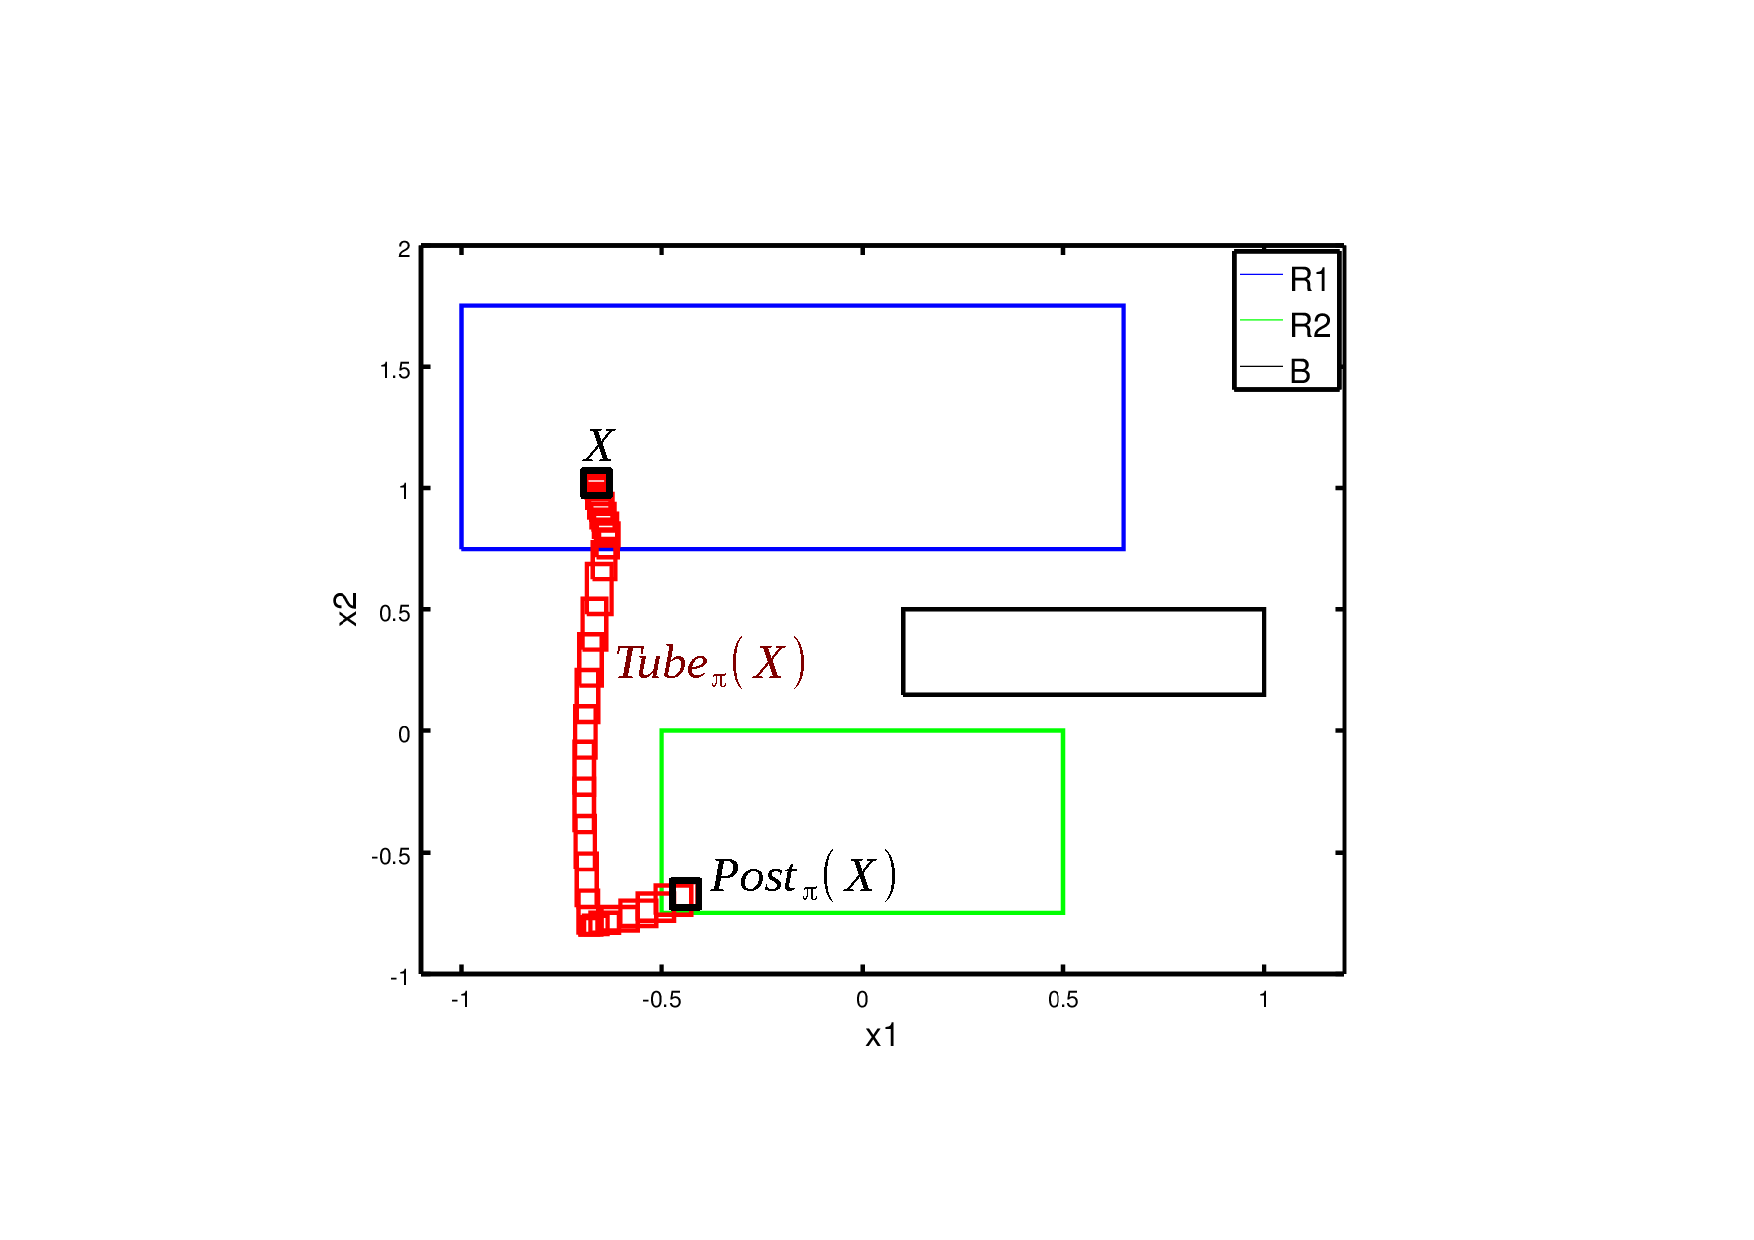
\includegraphics[%trim = 4cm 3cm 4cm 4cm, clip,
 width=0.5\textwidth]{tube.pdf}
 \caption{Functions $Post_{\pi}(X)$ and $Tube_{\pi}(X)$ for the
   initial box $X=[-0.69,-0.64] \times [1,1.06]$, with a pattern $\pi
   = (1,3,0)$.}
 \label{fig:post_tube}
\end{figure}

For a given pattern of switched modes $\pi = (i_1,\dots,i_k) \in U^k$
of length $k$, we are able to compute, for $j \in \{1,..,k\}$, the
enclosures:
\begin{itemize}
\item $[x_j] \ni x(j\tau)$;
\item $[\tilde{x}_j] \ni x(t), \ \text{for} \ t \in \lbrack
  (j-1)\tau,j\tau\rbrack$.
\end{itemize}
with respect to the system of IVPs:
\begin{equation}
  \left\{
    \begin{array}{c}
      \dot x(t) = f_{\sigma (t)}(t,x(t),d(t)),\\
      \nonumber x(t_0=0) \in [x_0] , d(t) \in [d],\\
      \sigma(t) = i_1, \forall t \in [0,t_1], t_1=\tau\\
      \vdots\\
      \dot x(t) = f_{\sigma (t)}(t,x(t),d(t)),\\
      \nonumber x(t_{k-1}) \in [x_{k-1}], d(t) \in [d],\\
      \sigma(t) = i_k, \forall t \in [t_{k-1},t_k], t_k=k\tau
    \end{array}
  \right.
\end{equation}
Thereby, the enclosure $Post_{\pi}(\lbrack x_0 \rbrack)$ is included
in $[x_k]$ and $Tube_{\pi}(\lbrack x_0 \rbrack)$ is included in
$\bigcup_{j=1,..,k} [\tilde{x}_j]$. This applies for all initial
states in $\lbrack x_0 \rbrack$ and all disturbances $d(t) \in [d]$. A
view of enclosures computed by the validated simulation for one
solution obtained for Example~\ref{ex2} is shown in
Figure~\ref{fig:post_tube}.



\subsubsection{Control synthesis}

If we now associate computation of the Post and Tube operators
to Algorithm \ref{algo:decomposition} and \ref{algo:findpattern2}, 
and using Theorem \ref{th:RS-procedure}, we can now perform control synthesis
ensuring $(R,S)$-stability, as well as $(R_1,R_2,S)$-reachability
and $(R,B,S)$-avoidance. 


\subsection{Experimentations}
\label{sec:experimentations}
%
In this subsection, we apply our approach to different case studies taken
from the literature.  Our solver prototype is written in C++ and based
on DynIBEX \cite{dynibex}.  The computations times given in the
following have been performed on a 2.80 GHz Intel Core i7-4810MQ CPU
with 8 GB of memory. Note that our algorithm is mono-threaded so all
the experimentation only uses one core to perform the computations.
The results given in this subsection have been obtained with Function
$Find\_Pattern2$.

\subsubsection{A linear example: boost DC-DC converter}

This linear example is taken from \cite{beccuti2005optimal} and has
already been treated with the state-space bisection method in a linear
framework in \cite{fribourg2014finite}. This running example is used to verify that our
approach is still valid for linear case, and also to show the strong improvement in term of computation time.

The system is a boost DC-DC converter with one switching cell.  There
are two switching modes depending on the position of the switching
cell. The dynamics is given by the equation $\dot x (t) =
A_{\sigma(t)} x(t) + B_{\sigma(t)}$ with $\sigma(t) \in U = \{ 1,2
\}$. The two modes are given by the matrices:

\begin{displaymath}
  A_1 = \left( \begin{matrix}
      - \frac{r_l}{x_l} & 0 \\ 0 & - \frac{1}{x_c} \frac{1}{r_0 + r_c}
    \end{matrix} \right)  \quad B_1 = \left( \begin{matrix}
      \frac{v_s}{x_l} \\ 0 \end{matrix} \right)
\end{displaymath}

\begin{displaymath}
  A_2 = \left( \begin{matrix} - \frac{1}{x_l} (r_l +
      \frac{r_0.r_c}{r_0 + r_c}) & - \frac{1}{x_l} \frac{r_0}{r_0 + r_c}
      \\ \frac{1}{x_c}\frac{r_0}{r_0 + r_c} & - \frac{1}{x_c}
      \frac{r_0}{r_0 + r_c}
    \end{matrix} \right)  \quad B_2 = \left( \begin{matrix}
      \frac{v_s}{x_l} \\ 0 \end{matrix} \right)
\end{displaymath}
with $x_c = 70$, $x_l = 3$, $r_c = 0.005$, $r_l = 0.05$, $r_0 = 1$,
$v_s = 1$.  The sampling period is $\tau = 0.5$.  The parameters are
exact and there is no perturbation.  We want the state to return
infinitely often to the region $R$, set here to $\lbrack 1.55 , 2.15
\rbrack \times \lbrack 1.0 , 1.4 \rbrack$, while never going out of
the safety set $S = \lbrack 1.54 , 2.16 \rbrack \times \lbrack 0.99 ,
1.41 \rbrack$.  The goal of this example is then to synthesize a
controller with intrinsic stability.

The decomposition was obtained in less than one second with a maximum
length of pattern set to $K = 6$ and a maximum bisection depth of $D =
3$.  A simulation is given in Figure~\ref{fig:NL_0}.

\begin{figure}[t]
 \centering
 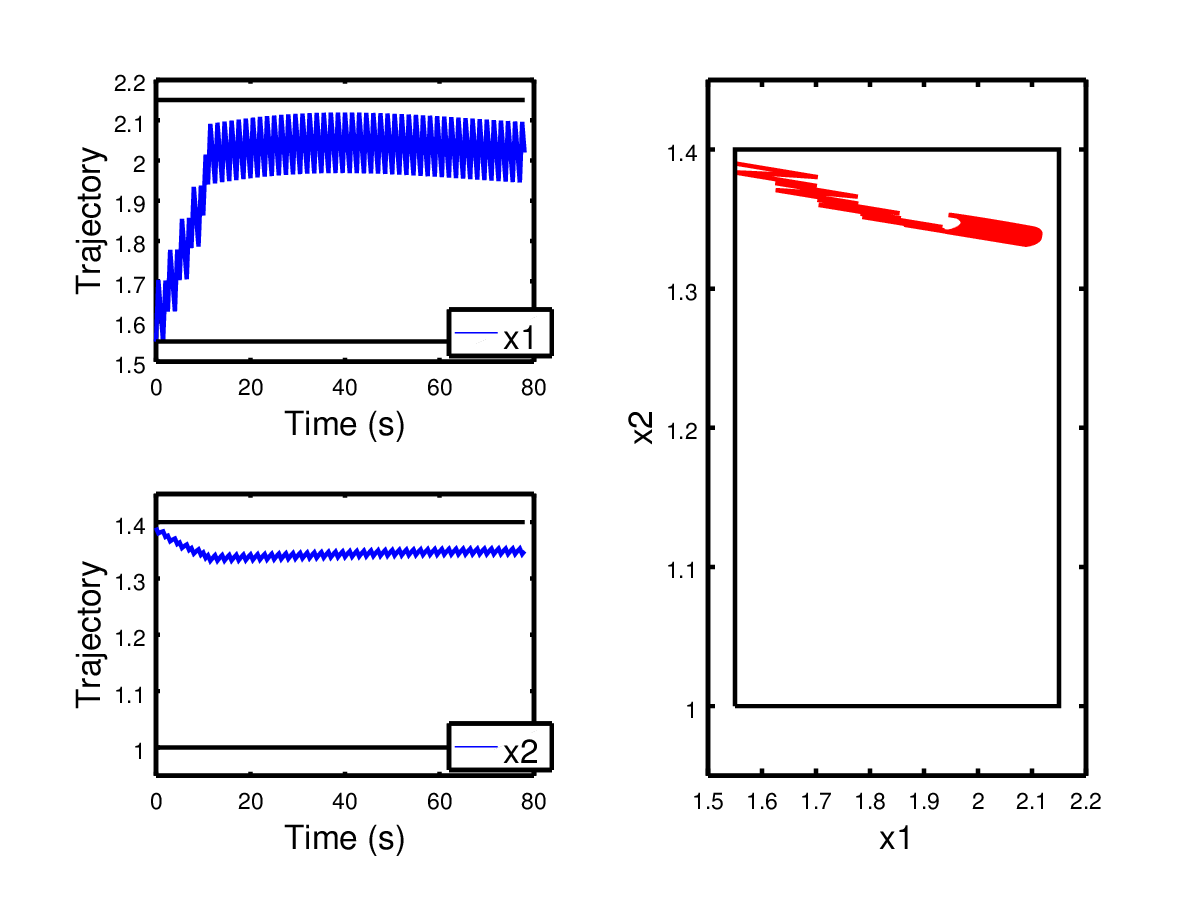
\includegraphics[scale=0.45]{simu_boost_safe.png}
 \caption{Simulation from the initial condition $(1.55,1.4)$. The box
   $R$ is in plain black. The trajectory is plotted within time for
   the two state variables on the left, and in the state-space plane
   on the right.}
  \label{fig:NL_0}
\end{figure}


\subsubsection{A polynomial example}
\label{ex2}
%
%
We consider the polynomial system taken from \cite{liu2013synthesis},
presented as a difficult example:
%
\begin{equation}
 \left \lbrack \begin{matrix}
  \dot x_1 \\ \dot x_2
 \end{matrix} \right \rbrack  =
 \left \lbrack \begin{matrix} -x_2 - 1.5 x_1 - 0.5 x_1^3 + u_1 + d_1 \\ x_1 + u_2 + d_2
   \end{matrix} \right \rbrack.
\end{equation}
%
The control inputs are given by $u = (u_1,u_2) =
K_{\sigma(t)}(x_1,x_2)$, $\sigma(t) \in U = \{ 1,2,3,4 \}$, which
correspond to four different state feedback controllers $K_1(x) =
(0,-x_2^2 + 2)$, $K_2(x) = (0,-x_2)$, $K_3(x) = (2,10)$, $K_4(x) =
(-1.5,10)$.  We thus have four switching modes. The disturbance $d =
(d_1,d_2)$ lies in $\lbrack -0.005,0.005 \rbrack \times \lbrack
-0.005,0.005 \rbrack$.  The objective is to visit infinitely often two
zones $R_1$ and $R_2$, without going out of a safety zone $S$, and
while never crossing a forbidden zone $B$.  Two decompositions are
performed:
\begin{itemize}
\item a decomposition of $R_1$ which returns $\{ (V_i,\pi_i) \}_{i
    \in I_1}$ with:
  \begin{itemize}
  \item $\bigcup_{i \in I_1} V_i = R_1$,
  \item $\forall i \in I_1, \ Post_{\pi_i}(V_i) \subseteq R_2$,
  \item $\forall i \in I_1, \ Tube_{\pi_i}(V_i) \subseteq S$,
  \item $\forall i \in I_1, \ Tube_{\pi_i}(V_i) \bigcap B = \emptyset$.
  \end{itemize}
\item a decomposition of $R_2$ which returns $\{ (V_i,\pi_i) \}_{i \in
    I_2}$ with:
  \begin{itemize}
  \item $\bigcup_{i \in I_2} V_i = R_2$,
  \item $\forall i \in I_2, \ Post_{\pi_i}(V_i) \subseteq R_1$,
  \item $\forall i \in I_2, \ Tube_{\pi_i}(V_i) \subseteq S$,
  \item $\forall i \in I_2, \ Tube_{\pi_i}(V_i) \bigcap B = \emptyset$.
  \end{itemize}
\end{itemize}

The input boxes are the following:
\begin{itemize}
\item $R_1 = \lbrack -0.5 , 0.5 \rbrack \times \lbrack -0.75 , 0.0
  \rbrack$,
\item $R_2 = \lbrack -1.0 , 0.65 \rbrack \times \lbrack 0.75 , 1.75
  \rbrack$,
\item $S = \lbrack -2.0 , 2.0 \rbrack \times \lbrack -1.5 , 3.0
  \rbrack$,
\item $B = \lbrack 0.1 , 1.0 \rbrack \times \lbrack 0.15 , 0.5
  \rbrack$.
\end{itemize}
The sampling period is set to $\tau = 0.15$. The decompositions were
obtained in $2$ minutes and $30$ seconds with a maximum length of
pattern set to $K = 12$ and a maximum bisection depth of $D = 5$.  A
simulation is given in Figure~\ref{fig:NL_1} in which the disturbance
$d$ is chosen randomly in $\lbrack -0.005,0.005 \rbrack \times \lbrack
-0.005,0.005 \rbrack$ at every time step.

\begin{figure}[t]
 \centering
 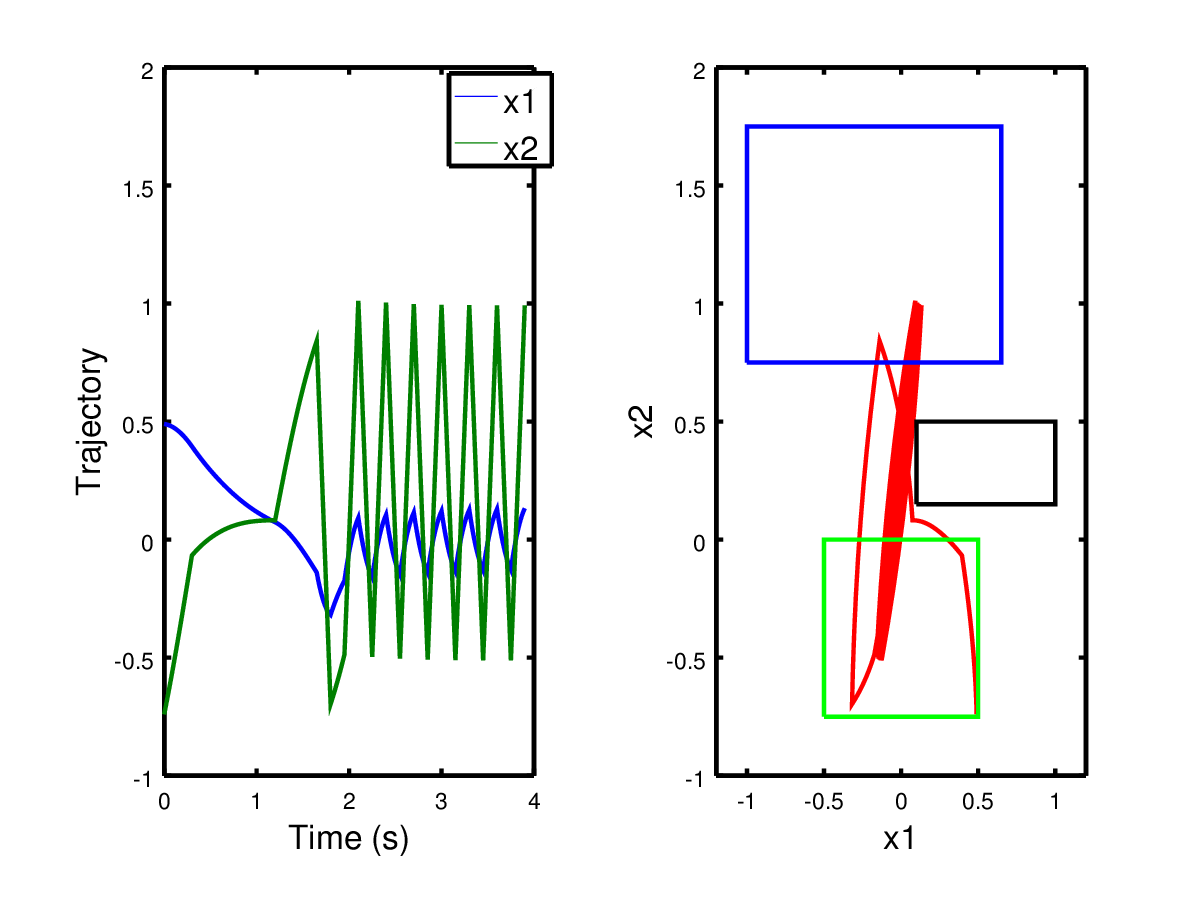
\includegraphics[scale=0.4]{simu_obstacle5.png}
 \caption{Simulation from the initial condition $(0.5,-0.75)$. The
   trajectory is plotted within time on the left, and in the state
   space plane on the right.  In the sate space plane, the set $R_1$
   is in plain green, $R_2$ in plain blue, and $B$ in plain black.}
 \label{fig:NL_1}
\end{figure}

\subsubsection{Building ventilation}
%
We consider a building ventilation application adapted from
\cite{meyer:tel-01232640}.  The system is a four room apartment
subject to heat transfer between the rooms, with the external
environment, with the underfloor, and with human beings.  The dynamics
of the system is given by the following equation:
\begin{displaymath}
 \frac{d T_i}{dt} = \sum_{j \in \mathcal{N}^\text{*}\setminus \{i\}} a_{ij} (T_j -
 T_i) + \delta_{s_i} b_i (T_{s_i}^4 - T_i ^4 ) + c_i
 \max\left(0,\frac{V_i - V_i^\text{*}}{\bar{ V_i} -
   V_i^{\text{*}}}\right)(T_u - T_i).
\end{displaymath}

The state of the system is given by the temperatures in the rooms
$T_i$, for $i \in \mathcal{N} = \{ 1 , \dots , 4 \}$.  Room $i$ is
subject to heat exchange with different entities stated by the indexes
$\mathcal{N}^\text{*} = \{1,2,3,4,u,o,c \}$.

\begin{figure}[t]
  \centering
  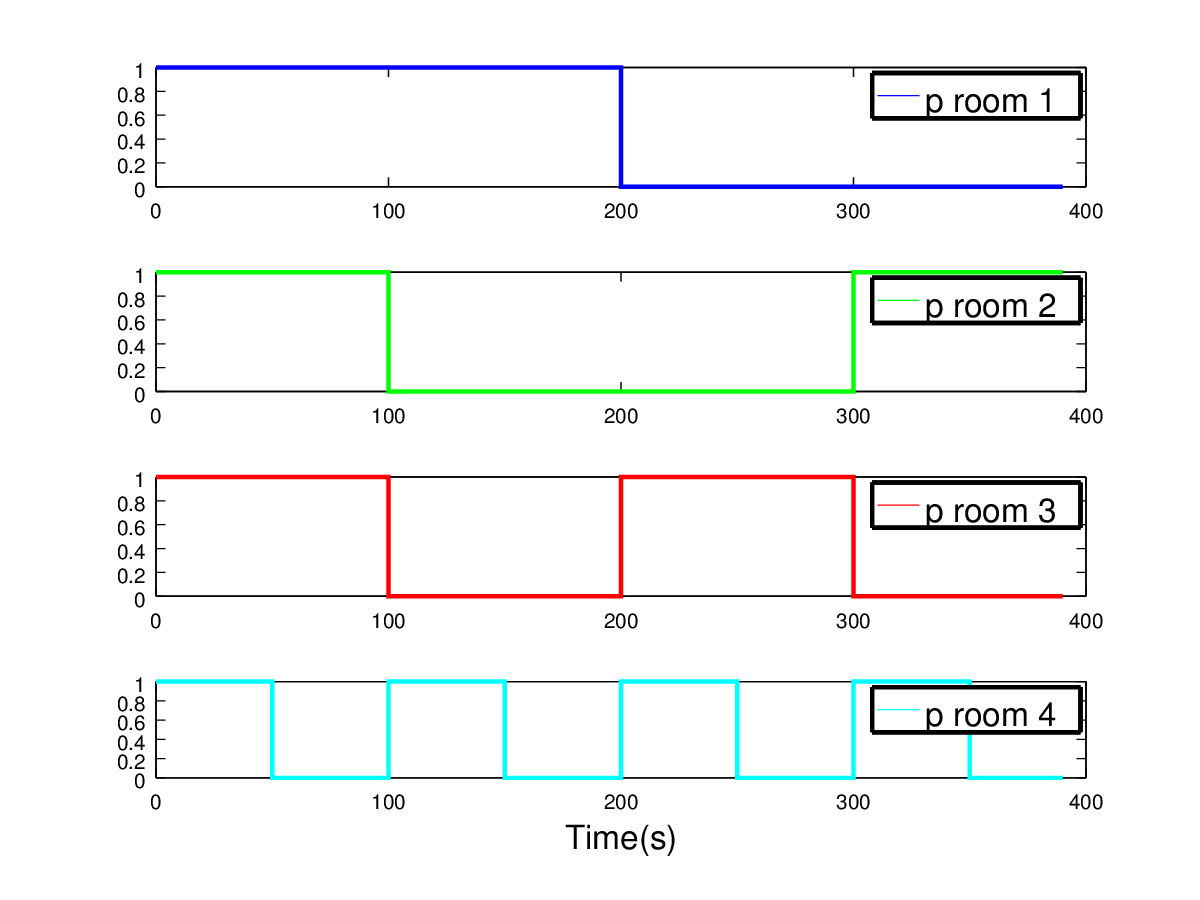
\includegraphics[scale=0.4]{NL_case_2_perturbation.png}
  \caption{Perturbation (presence of humans) imposed within time in the
    different rooms.}
  \label{fig:NL_2_perturbation}
\end{figure}


The heat transfer between the rooms is given by the coefficients
$a_{ij}$ for $i,j \in \mathcal{N}^2$, and the different perturbations
are the following:
\begin{itemize}
 \item The external environment: it has an effect on room $i$ with the
   coefficient $a_{io}$ and the outside temperature $T_o$, varying
   between $27^\circ C$ and $30^\circ C$.
  \item The heat transfer through the ceiling: it has an effect on
    room $i$ with the coefficient $a_{ic}$ and the ceiling temperature
    $T_c$, varying between $27^\circ C$ and $30^\circ C$.
  \item The heat transfer with the underfloor: it is given by the
    coefficient $a_{iu}$ and the underfloor temperature $T_u$, set to
    $17^\circ C$ ($T_u$ is constant, regulated by a PID controller).
  \item The perturbation induced by the presence of humans: it is
    given in room $i$ by the term $\delta_{s_i} b_i (T_{s_i}^4 - T_i
    ^4 )$, the parameter $\delta_{s_i}$ is equal to $1$ when someone
    is present in room $i$, $0$ otherwise, and $T_{s_i}$ is a given
    identified parameter.
\end{itemize}

\begin{figure}[t]
  \centering
  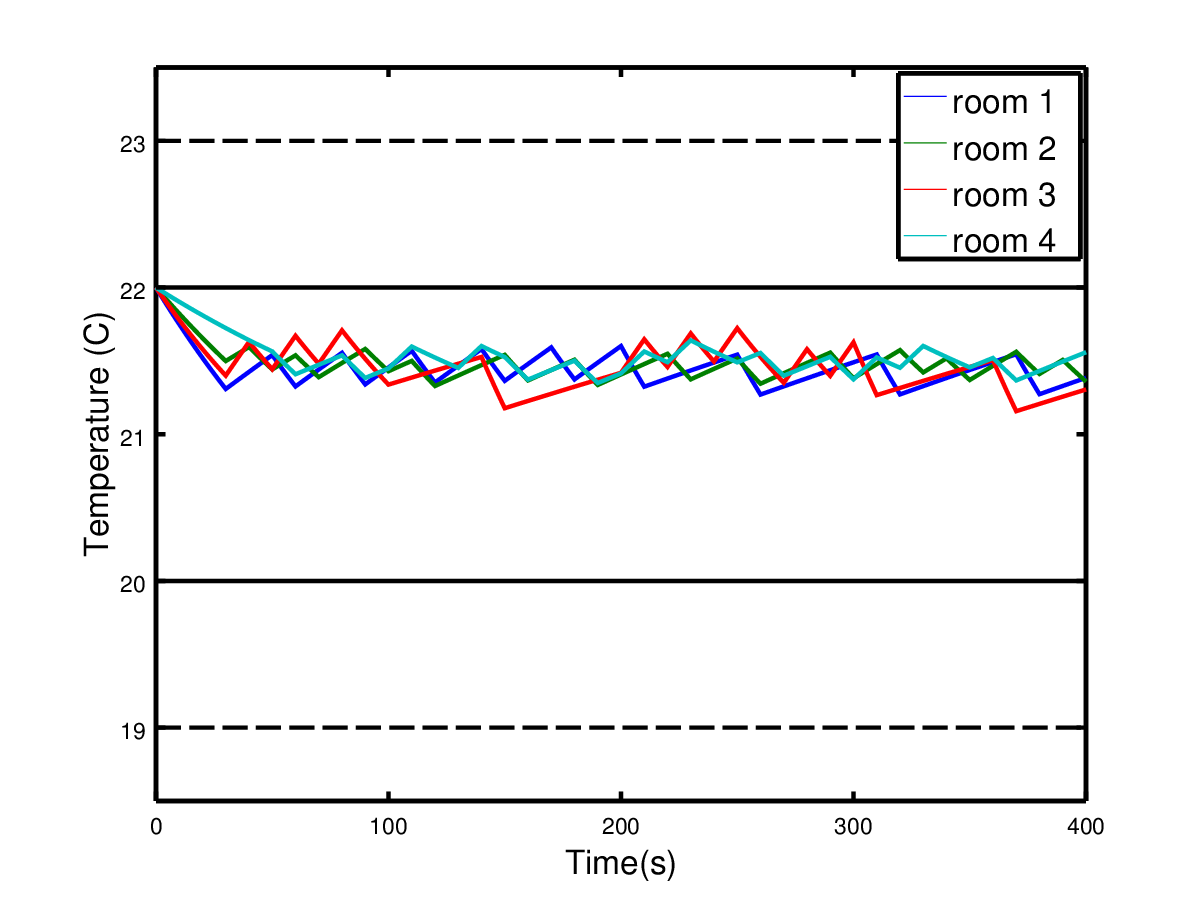
\includegraphics[scale=0.4]{NL_case_2.png}
  \caption{Simulation from the initial condition $(22,22,22,22)$. The
    objective set $R$ is in plain black and the safety set $S$ is in
    dotted black.}
  \label{fig:NL_2}
\end{figure}

The control $V_i$, $i \in \mathcal{N}$, is applied through the term
$c_i \max(0,\frac{V_i - V_i^\text{*}}{\bar{ V_i} -
  V_i^{\text{*}}})(T_u - T_i)$.  A voltage $V_i$ is applied to force
ventilation from the underfloor to room $i$, and the command of an
underfloor fan is subject to a dry friction.  Because we work in a
switched control framework, $V_i$ can take only discrete values, which
removes the problem of dealing with a ``max'' function in interval
analysis. In the experiment, $V_1$ and $V_4$ can take the values $0$V
or $3.5$V, and $V_2$ and $V_3$ can take the values $0$V or $3$V. This
leads to a system of the form of Equation~\eqref{eq:sys} with
$\sigma(t) \in U =\{ 1, \dots, 16 \}$, the $16$ switching modes
corresponding to the different possible combinations of voltages
$V_i$.  The sampling period is $\tau = 10$s.

The parameters $T_{s_i}$, $V_i^\text{*}$, $\bar V_i$, $a_{ij}$, $b_i$,
$c_i$ are given in \cite{meyer:tel-01232640} and have been identified
with a proper identification procedure detailed in
\cite{meyer2014ecc}.  Note that here we have neglected the term
$\sum_{j \in \mathcal{N}} \delta_{d_{ij}}c_{i,j} \ast h(T_j - T_i)$ of
\cite{meyer:tel-01232640}, representing the perturbation induced by
the open or closed state of the doors between the rooms. Taking a
``max'' function into account with interval analysis is actually still
a difficult task. However, this term could have been taken into
account with a proper regularization (smoothing).

The main difficulty of this example is the large number of modes in
the switched system, which induces a combinatorial issue.

The decomposition was obtained in $4$ minutes with a maximum length of
pattern set to $K = 2$ and a maximum bisection depth of $D = 4$.  The
perturbation due to human beings has been taken into account by
setting the parameters $\delta_{s_i}$ equal to the whole interval
$\lbrack 0,1 \rbrack$ for the decomposition, and the imposed
perturbation for the simulation is given
Figure~\ref{fig:NL_2_perturbation}.  The temperatures $T_o$ and $T_c$
have been set to the interval $\lbrack27,30\rbrack$ for the
decomposition, and are set to $30^\circ C$ for the simulation.  A
simulation of the controller obtained with the state-space bisection
procedure is given in Figure~\ref{fig:NL_2}, where the control
objective is to stabilize the temperature in $\lbrack 20 , 22 \rbrack
^4$ while never going out of $\lbrack 19 , 23 \rbrack ^4$.

\subsubsection{A path planning problem}


This last case study is based on a model of a vehicle initially
introduced in \cite{astrom2010feedback} and successfully controlled in
\cite{zamani2012symbolic,reissig2015feedback} with the tools PESSOA
and SCOTS. In this model, the motion of the front and rear pairs of
wheels are approximated by a single front wheel and a single rear
wheel. The dynamics if the vehicle is given by:
\begin{equation}
 \begin{array}{ccc}
  \dot x & = & v_0 \frac{\cos(\alpha + \theta)}{\cos(\alpha)} \\
  \dot y & = & v_0 \frac{\sin(\alpha + \theta)}{\cos(\alpha)} \\
  \dot \theta & = & \frac{v_0}{b} \tan(\delta)
  \end{array}
\end{equation}
where $\alpha = \arctan( a \tan (\delta) / b)$. The system is thus of
dimension $3$, $(x,y)$ is the position of the vehicle, while $\theta$
is the orientation of the vehicle.  The control inputs are $v_0$, an
input velocity, and $\delta$, the steering angle of the rear wheel.
The parameters are: $a=0.5$, $b=1$.  Just as in
\cite{zamani2012symbolic,reissig2015feedback}, we suppose that the
control inputs are piecewise constant, which leads to a switched
system of the form of Equation~\eqref{eq:sys} with no perturbation.
The objective is to send the vehicle into an objective region $R_2 =
[9,9.5]\times[0,0.5]\times ]-\infty,+\infty[$ from an initial region
$R_1 = [0,0.5]\times[0,0.5]\times[0,0]$. The safety set is $S = [0,10]
\times [0,10] \times]-\infty,+\infty[$.  There is in fact no
particular constraint on the orientation of the vehicle, but multiple
obstacles are imposed for the two first dimensions, they are
represented in Figure \ref{fig:unicycle}. The input velocity $v_0$ can
take the values in $\{-0.5,0.5,1.0\}$. The rear wheel orientation
$\delta$ can take the values in
$\{0.9,0.6,0.5,0.3,0.0,-0.3,-0.5,-0.6,-0.9\}$. The sampling period is
$\tau = 0.3$.

\begin{figure}[t]
  \centering
  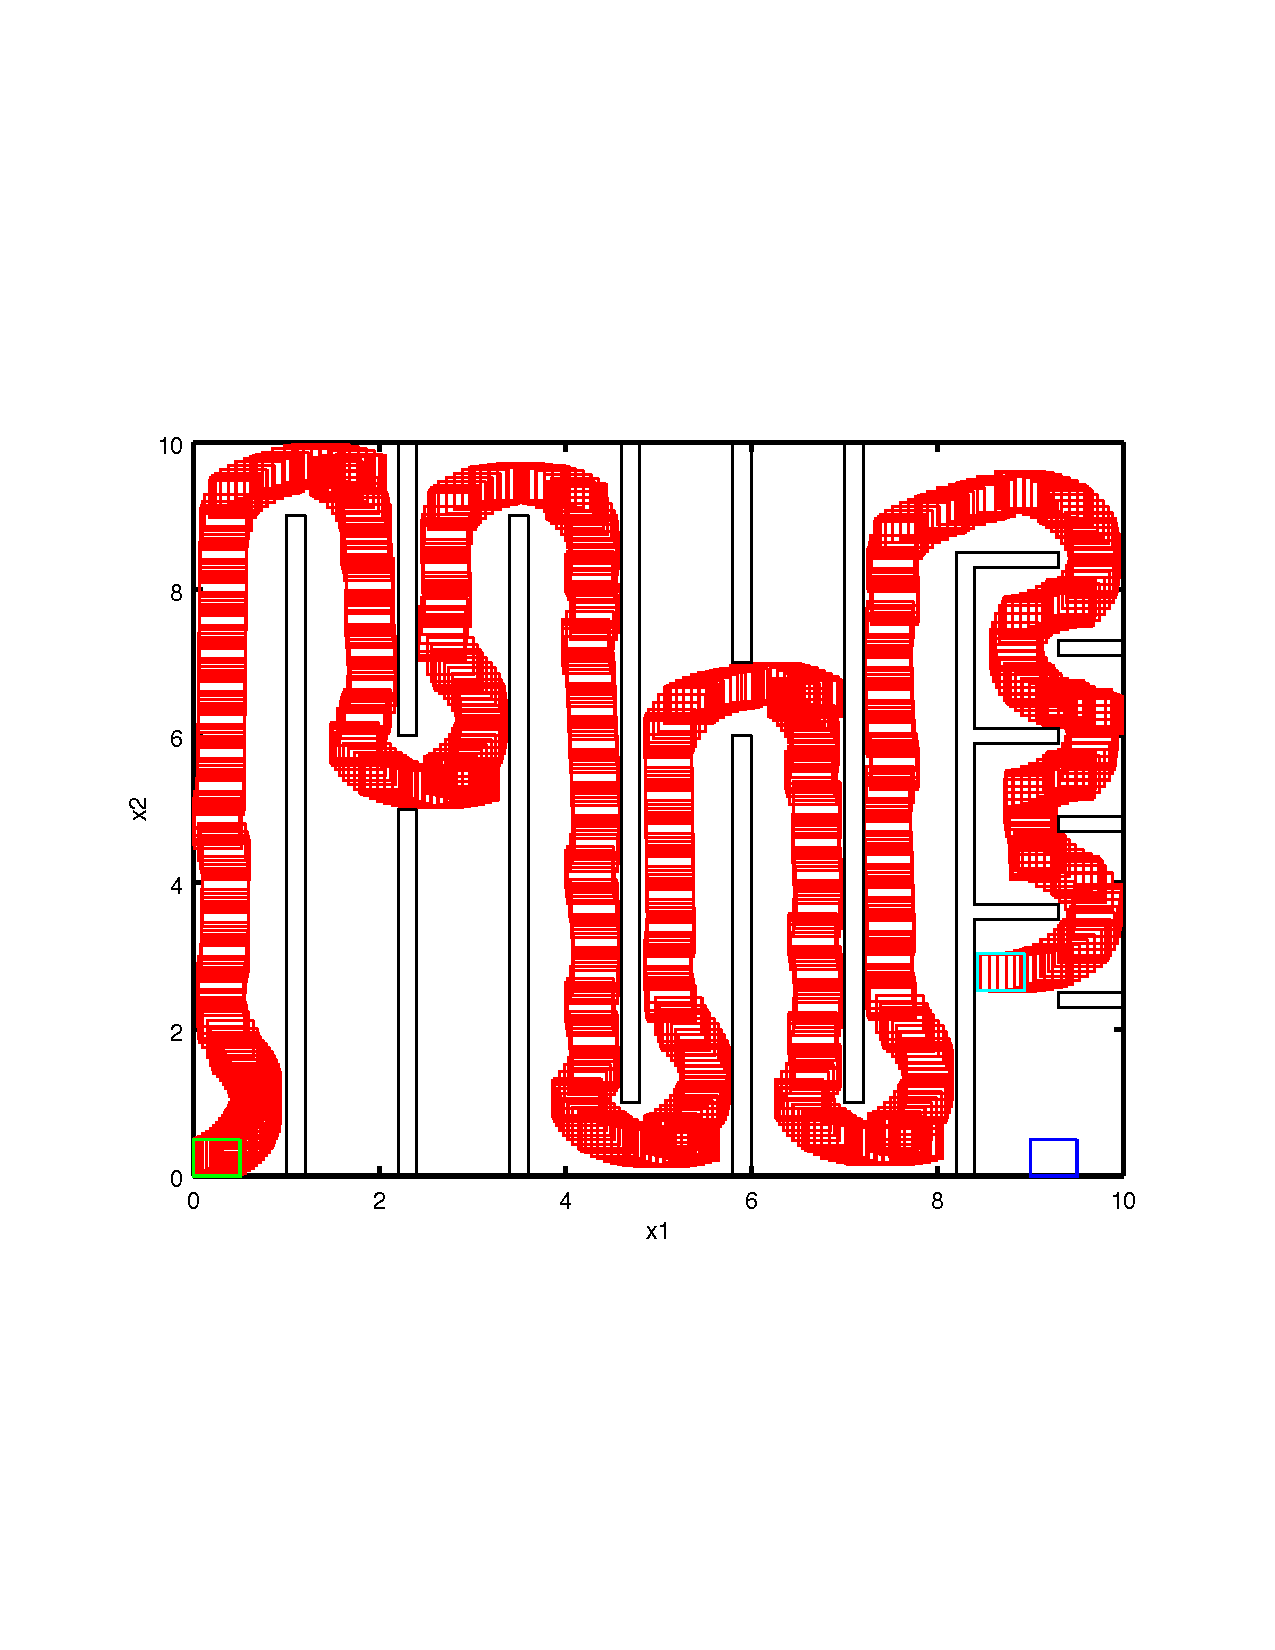
\includegraphics[scale=0.5% ,clip,trim=0cm 6.5cm 0cm 6.5cm
  ]{unicycle_sol.pdf}
  \caption{Set simulation of the path planning example. The green box
    is the initial region $R_1$, the blue box is the target region
    $R_2$. The union of the red boxes is the reachability tube. In
    this case, the target region is not attained without bisection.}
  \label{fig:unicycle}
\end{figure}


\begin{figure}[t]
  \centering
  \begin{tabular}{cc}
    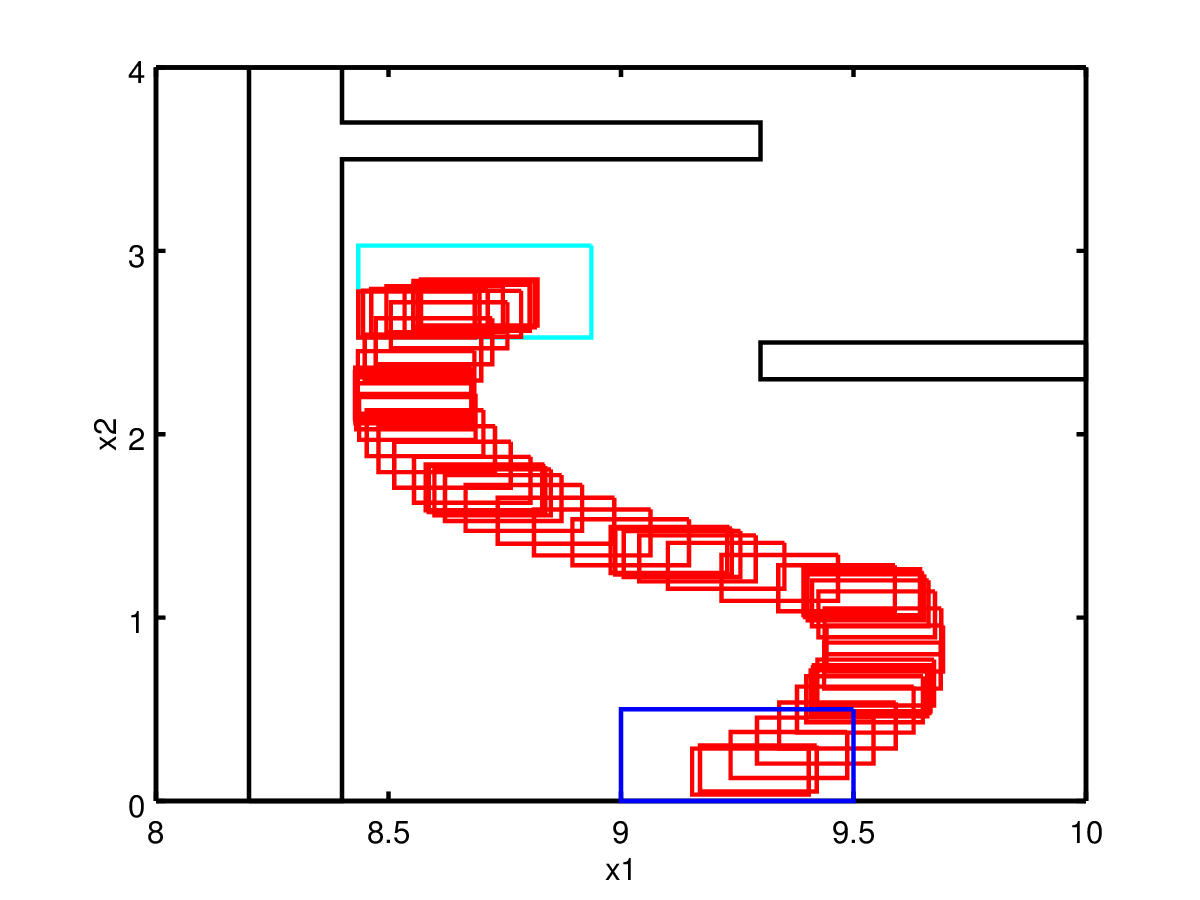
\includegraphics[width=0.35\textwidth,clip,trim=0cm 0cm 0cm 0cm]{uni1.png}
    &
    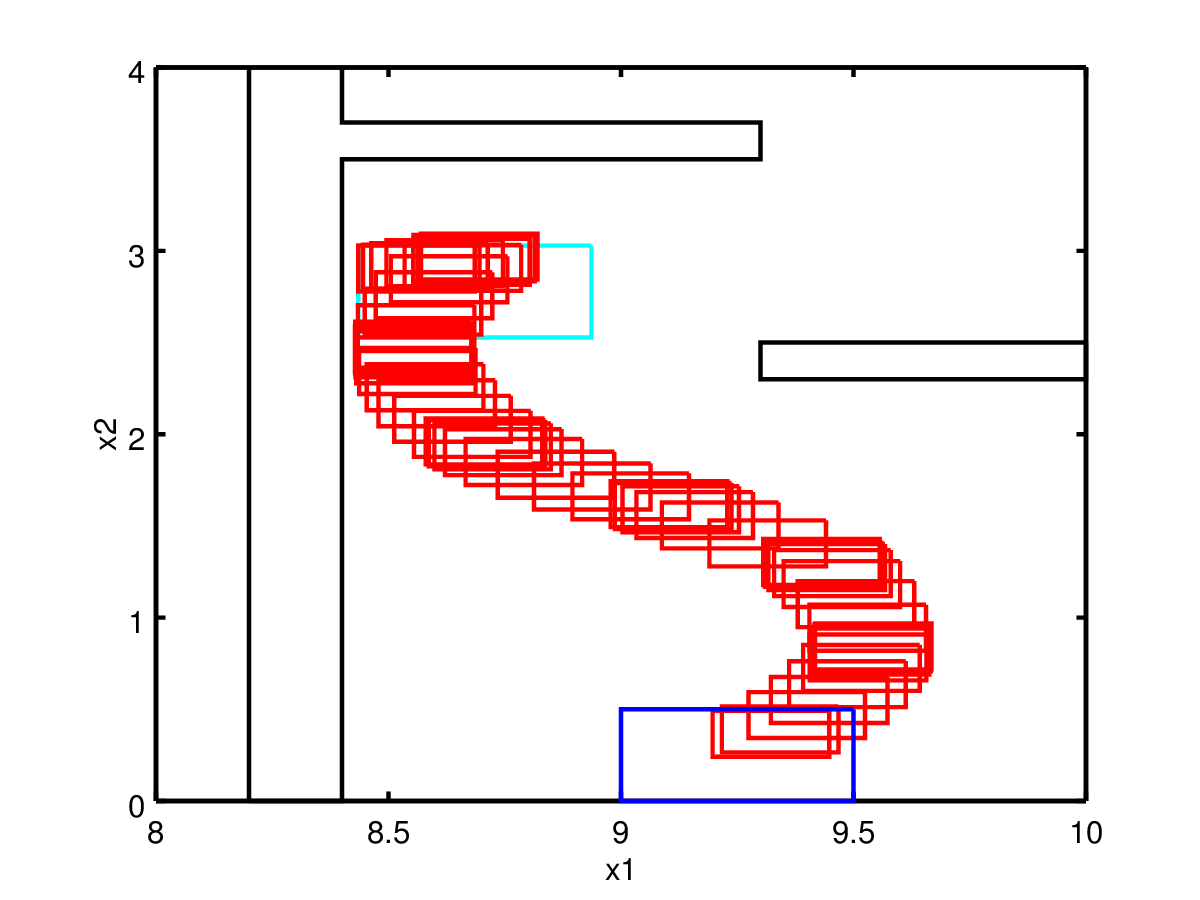
\includegraphics[width=0.35\textwidth,clip,trim=0cm 0cm 0cm 0cm]{uni2.png}
    \\
    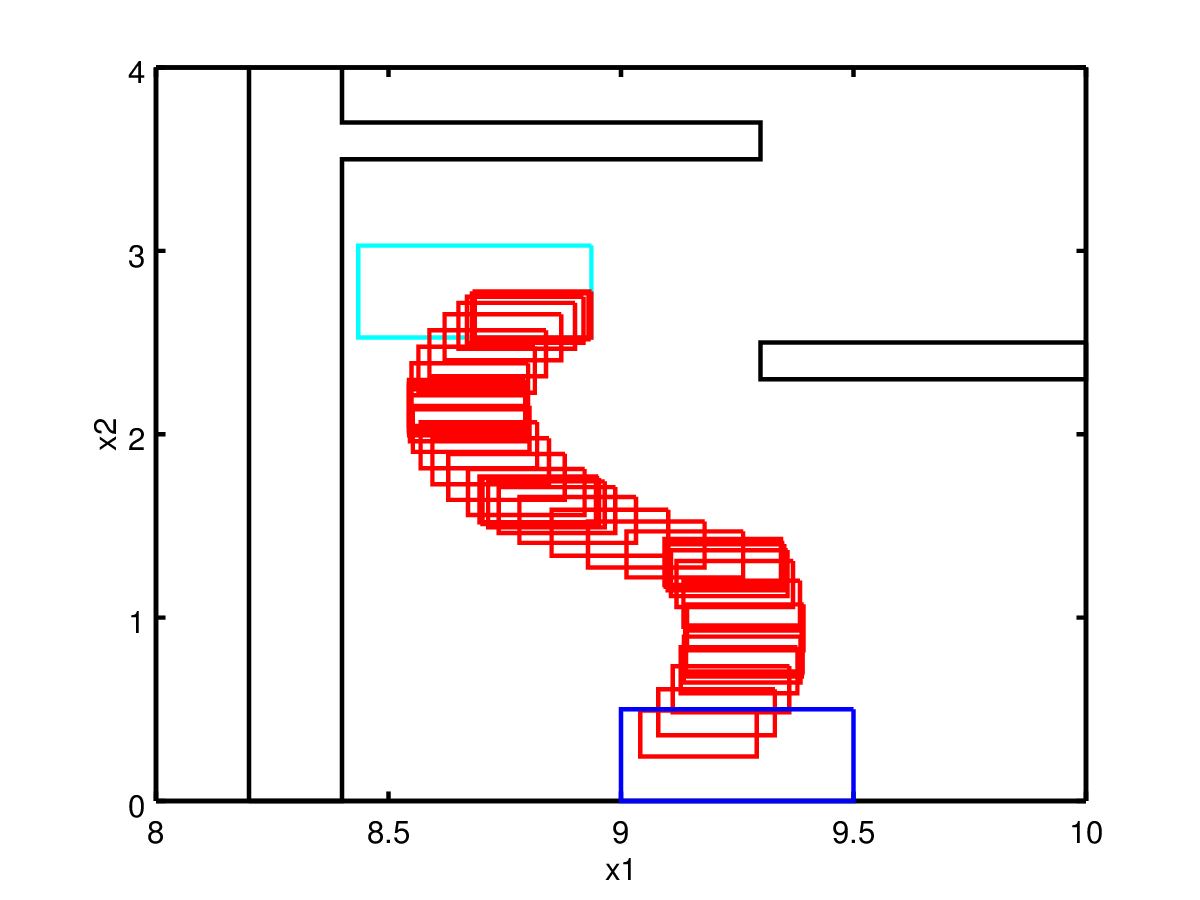
\includegraphics[width=0.35\textwidth,clip,trim=0cm 0cm 0cm 0cm]{uni3.png}
    &
    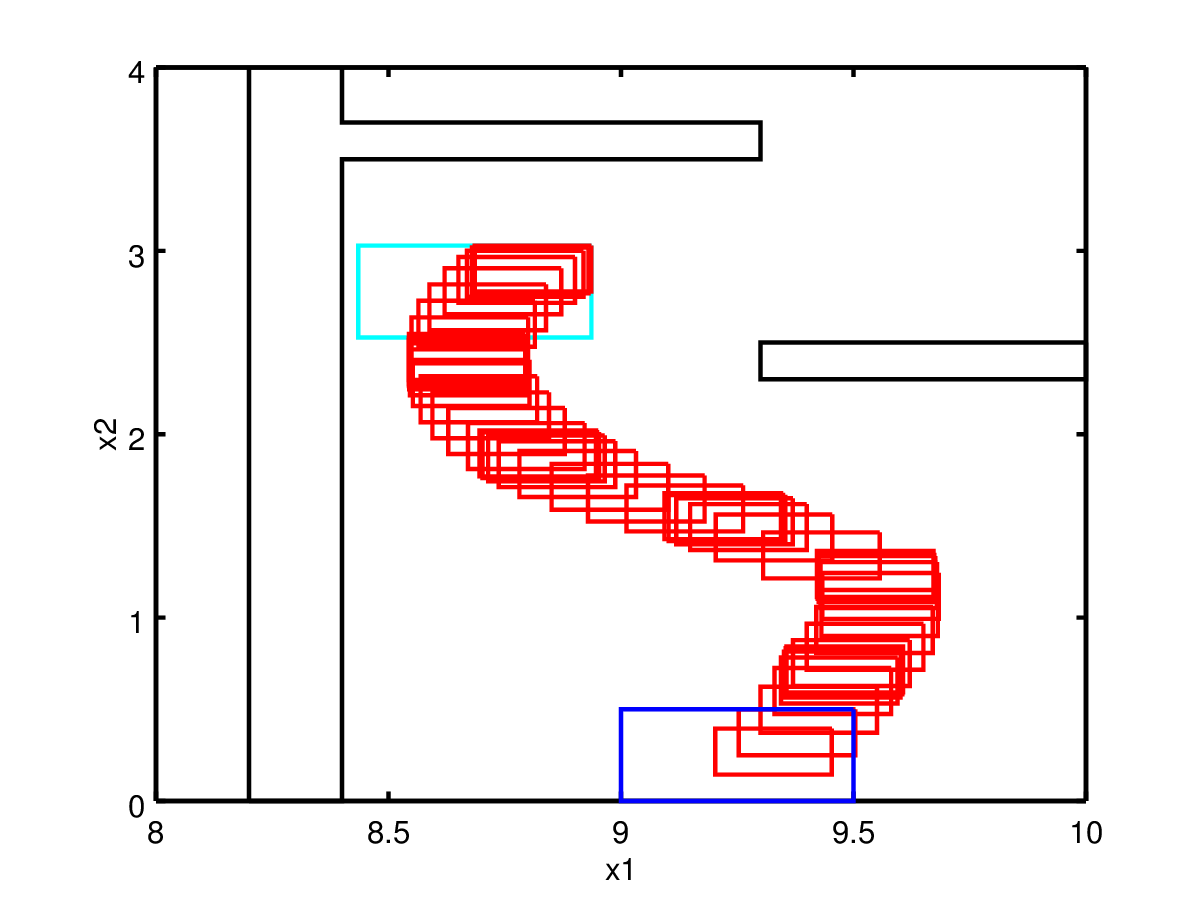
\includegraphics[width=0.35\textwidth,clip,trim=0cm 0cm 0cm 0cm]{uni4.png}
  \end{tabular}
  \caption{Set simulation of the path planning example after
    bisection. The green boxes are the initial regions obtained by
    bisection, the blue box is the target region $R_2$. The union of
    the red boxes is the reachability tube.}
  \label{fig:unicycle2}
\end{figure}


Note that for this case study we used an automated pre-tiling of the
state-space permitting to decompose the reachability problem in a
sequence of reachability problems.  Using patterns of length up to
$K=10$, we managed to successfully control the system in $3619$
seconds. In this case, the pattern is computed until almost the end
without bisection as shown in Figure~\ref{fig:unicycle}. To obtain the
last steps, the box is bissected in four ones by
Algorithm~\ref{algo:decomposition}. After that, patterns are found for
the four boxes:
\begin{itemize}
 \item $[8.43, 8.69] ; [2.52, 2.78] : \{7 0 0 0 1 6 6 \}$
 \item $[8.43, 8.69] ; [2.78, 3.03] : \{7 0 0 0 2 5 6 \}$
 \item $[8.69, 8.94] ; [2.52, 2.78] : \{0 0 0 5 5 \}$
 \item $[8.69, 8.94] ; [2.78, 3.03] : \{0 0 0 2 6 5 \}$
\end{itemize}

The four set simulations obtained for the last steps are given in
Figure~\ref{fig:unicycle2}.


\subsection{Performance tests}
\label{sec:comparison}

We present a comparison of functions $Find\_Pattern$, $Find\_Pattern2$
w.r.t. the computation times obtained, and with the state-of-the-art
tools PESSOA \cite{Mazo2010} and SCOTS \cite{SCOTS}.


Table~\ref{tab:FP1-FP2} shows a comparison of functions
$Find\_Pattern$ and $Find\_Pattern2$, which shows that the new version
highly improves computation time.  We can note that the new
version is all the more efficient as the length of the patterns
increases, and as obstacles cut the research tree of patterns. This is
why we observe significant improvements on the examples of the DC-DC
converter and the polynomial example, and not on the building
ventilation example, which only requires patterns of length $2$, and
presents no obstacle.

\begin{table}[t]
  \centering
  \caption{Comparison of $Find\_Pattern$ and $Find\_Pattern2$.}
  \label{tab:FP1-FP2}
  \begin{tabular}{|c|c|c|}
    \hline
    Example & \multicolumn{2}{c|}{Computation time} \\
    \cline{2-3} & $~Find\_Pattern~$ & $~Find\_Pattern2~$   \\
    \hline
    DC-DC Converter &    $1609$ s  &  $< 1$ s \\
    Polynomial example & Time Out   & $150$ s  \\
    Building ventilation & $272$ s & $228$ s  \\
    Path planning & Time Out & $3619$ s \\
    \hline
  \end{tabular}
\end{table}

Table~\ref{tab:SOTA} shows of comparison of function $Find\_Pattern2$
with state-of-the-art tools SCOTS and PESSOA.  On the example of the
DC-DC converter, our algorithm manages to control the whole
state-space $R=\lbrack 1.55 , 2.15 \rbrack \times \lbrack 1.0 , 1.4
\rbrack$ in less than one second, while SCOTS and PESSOA only control
a part of $R$, and with greater computation times. Note that these
computation times vary with the number of discretization points used
in both, but even with a very fine discretization, we never managed to
control the whole box $R$.  For the polynomial example, we manage to
control the whole boxes $R_1$ and $R_2$, such as SCOTS and in a
comparable amount of time. However, PESSOA does not support natively
this kind of nonlinear systems. For path planning case study, on which
PESSOA and SCOTS perform well, we have not obtained as good
computations times as they have.  This comes from the fact that this
example requires a high number of switched modes, long patterns, as
well as a high number of boxes to tile the state-space.  This is in
fact the most difficult case of application of our method.  This
reveals that our method is more adapted when either the number of
switched modes of the length of patterns is not high (though it can be
handled at the cost of high computation times).  Another advantage is
that we do not require a homogeneous discretization of the state
space. We can thus tile large parts of the state-space using only few
boxes, and this often permits to consider much less symbolic states
than with discretization methods, especially in higher dimensions (see
\cite{LeCoent2016}).


\begin{table}[t]
  \centering
  \caption{Comparison with state-of-the-art tools.}
  \label{tab:SOTA}
  \begin{tabular}{|c|c|c|c|}
    \hline
    Example & \multicolumn{3}{c|}{Computation time} \\
    \cline{2-4} & ~FP2~ & ~SCOTS~ & ~PESSOA~   \\
    \hline
    DC-DC Converter & $< 1$ s &    $43$ s  &  $760$ s \\
    Polynomial example & $150$ s & $131$ s & $\_\_$  \\
    Path planning & $3619$ s & $492$ s & $516$ s \\
    \hline
  \end{tabular}
\end{table}


\subsection{Conclusion}
\label{sec:conclu}

We presented a method of control synthesis for nonlinear switched
systems, based on a simple state-space bisection algorithm, and on
validated simulation. The approach permits to deal with stability,
reachability, safety and forbidden region constraints. Varying
parameters and perturbations can be easily taken into account with
interval analysis. The approach has been numerically validated on
several examples taken from the literature, a linear one with constant
parameters, and two nonlinear ones with varying perturbations.  Our
approach compares well with the state-of-the art tools SCOTS and
PESSOA.

We would like to point out that the exponential complexity of the
algorithms presented here, which is inherent to guaranteed methods, is
not prohibitive. Two approaches have indeed been developed to overcome
this exponential complexity.  A first approach is the use of
compositionality, which permits to split the system in two (or more)
sub-systems, and to perform control synthesis on these sub-systems of
lower dimensions.  This approach has been successfully applied in
\cite{LeCoent2016} to a system of dimension $11$, and we are currently
working on applying this approach to the more general context of
contract-based design \cite{sangiovanni2012taming}.  A second approach
is the use of Model Order Reduction, which allows to approximate the
full-order system \eqref{eq:sys} with a reduced-order system, of lower
dimension, on which it is possible to perform control synthesis.  The
bounding of the trajectory errors between the full-order and the
reduced-order systems can be taken into account, so that the induced
controller is guaranteed. This approach, described in
\cite{le2016control}, has been successfully applied on
(space-discretized) partial differential equations, leading to systems
of ODEs of dimension up to $100 000$.  The present work is a potential
ground for the application of such methods to control of nonlinear
partial differential equations, with the use of proper nonlinear model
order reduction techniques.




\section{Sampled switched systems with one-sided Lipschitz conditions}\label{sec:OSL}
\subsection{Lipschitz and one-sided Lipschitz condition}\label{ss:OSC}
Let us consider a nonlinear switched system of the form \eqref{eq:switched_system0}.
We make the following hypothesis:
%
$$(H0)\quad  \mbox{ For all  $j\in U$, $f_j$ is a locally Lipschitz continuous map}.$$
%
As in \cite{girard2010approximately}, we make the assumption that 
the vector field $f_j$ is such that the solutions of the 
differential equation  (\ref{eq:switched_system0}) are defined, 
e.g. by assuming that the support of the vector field $f_j$ is compact.
% We will denote by $\phi_\sigma(t;x^0)$ the 
% solution at time~$t$ of the system:
% 
% \begin{equation}
% \begin{aligned}
%   \dot x(t) & = f_{\sigma (t)}(x(t)), \\
%   x(0) & =  x^0. \\
% %  \sigma(t) & =  j \in U \ \text{for} \ t
% %  \in \lbrack k\tau , (k+1)\tau ),\ \ k=0,1,\dots
% \end{aligned}
%  \label{eq:ssampled-sys_part2}
% \end{equation}
%


%that the system is in a given mode $\sigma(t) =\sigma = j \in U$, 
%we abbreviate, for $t \in [0,\tau )$, $x_\sigma(t) = \phi(t;x^0,\sigma)$.
%%as well as $\tilde x_\sigma(t) = \tilde \phi_{\tilde x^0}(t;\tilde x^0,\sigma)$.

%\begin{remark}
%Definir $\phi$ pour pattern $\pi$ et $0\leq t <k\tau$ (ou $0\leq t \leq k\tau$).
%\end{remark}

We denote by $T$ a compact overapproximation of the image by $\phi_j$ of $S$ for $0\leq t\leq \tau$ and $j\in U$, i.e.~$T$ is such that
$$ T\supseteq \{\phi_j(t;x^0) \ |\ j\in U, 0\leq t\leq\tau, x^0\in S\}.$$
%%%%
The existence of $T$ is guaranteed by assumption $(H0)$. We know furthermore 
by $(H0)$ that, for all $j\in U$, there exists a constant $L_j>0$ such that:
%\label{hyp:2}
%For all $j \in U$, there exists a constant $L_j>0$ such that
\begin{equation}
\| f_j(y)-f_j(x) \| \leq L_j \, \|y-x\|\quad \forall x,y\in S.
\label{eq:lipschitz}
\end{equation}
Let us define $C_j$ for all $j\in U$:
%We have:
\begin{equation}
%L\|f_{j}(x)\|\leq C_0 
C_j = \sup_{x\in S}\  L_j\|f_j(x)\|
\quad
\text{for all} \quad j\in U.
\label{eq:L}
\end{equation}
%
We make the additional hypothesis 
that the mappings $f_j$ are {\em one-sided Lipschitz} (OSL)
\cite{Donchev98}.

%, which are often verified on systems modeling
%real world applications such as temperature regulation in a building (eg., \cite{meyer2014ecc}):
%we consider 
%%%The Lipschitz condition is classically assumed in order to 
% ensure the existence of a (unique) integral solution $\phi_\sigma$
%(see, e.g., \cite{liberzon2012switching}). 
%This assumption of strong monotony is original in the context of switched systems, as far as we know. 
Formally:
%
$$(H1) 
%\label{hyp:1}
\quad \mbox{ For all $j \in U$, there exists a constant $\lambda_j\in \mathbb{R}$ such that}$$ 
\[
\langle f_j(y)-f_j(x), y-x \rangle \leq \lambda_j\, \|y-x\|^2\quad
\forall x,y\in T,
\]
where $\langle \cdot, \cdot\rangle$ denotes the scalar product of two vectors of $\mathbb{R}^n$.
%\end{definition}
%
%\footnote{Let  $\lambda_{min} = \min_{j \in U} \lambda_j$.}
Constant $\lambda_j \in \R$ is called one-sided Lipschitz (OSL) constant, and can also be found in the 
literature as Dahlquist's constant [ref???].
Note that in practice, hypotheses H0 and H1 are not strong. 
Hypothesis H0 just ensures the existence of solutions for system,
and constants $L_j$ and $\lambda_j$ can always be found if the state 
of the system stays in a compact (e.g. the set $T$).
%have (in the case of linear equations) eigenvalues of very different modulus.
%The stability of systems governed by stiff equations is difficult to establish using only  Lipschitz constants.\footnote{The Euler method can also be numerically unstable, especially for stiff equations, meaning that the numerical solution grows very large for equations where the exact solution does not (Wikipedia).}
%

\paragraph{Computation of constants $\lambda_j$, $L_j$ and $C_j$}

The computation of constants $L_j$, $C_j$, $\lambda_j$ 
($j\in U$) are realized with
a constrained optimization algorithm.
They are performed using the ``sqp'' function of Octave, applied on the following 
optimization problems:
\begin{itemize}
 \item Constant $L_j$:
 $$ L_j = \max_{{x,y}\in S,\  x\neq y} \frac{\| f_j(y) - f_j(x) \|}{\| y - x \|}  $$
 \item Constant $C_j$:
 $$ C_j = \max_{{x}\in S} L_j \| f_j(x) \|$$
 \item Constant $\lambda_j$:
 $$ \lambda_j = \max_{{x,y}\in T,\  x\neq y} \frac{\langle f_j(y) - f_j(x), y - x \rangle}{\|y - x \|^2 }$$
 \end{itemize}
We could point out that the computation of the constants is not guaranteed, in the 
sense that the results given by optimization algorithms does not 
provide a guarantee that an overapproximation of the constants is computed. However,
some works have been done for computing over and under approximation
of Lipschitz constants in \cite{} [???], and could be used here. This approach can 
be extended to the OSL constant. In the following, we consider that we can 
compute these constants exactly.
 
 
\paragraph{Origin of the OSL property}

This notion has been used for the first time by \cite{donchev1998stability}
in order to treat ``stiff'' systems of differential equations for which the explicit Euler method is
numerically ``unstable'' (unless the step size is taken to be extremely small).
Unlike Lipschitz constants, OSL constants can be {\em negative}.
In the case where an OSL constant $\lambda_j$ is negative, it is said that the vector 
field $f_j$ is strongly monotone \cite{???},
which express a form of contractivity of the system dynamics: a strongly monotone system
presents trajectories getting exponentially closer together 
within time.
Even if the OSL constant is positive, it is in practice much lower than
the Lipschitz constant \cite{dahlquist1976error}. The use of OSL thus allows us to obtain a much
more precise upper bound for the global error.
We believe that this notion is also closely related to
the notion of incremental stability \cite{???}. We think that 
it could be shown that any system presenting a negative OSL constant is
incrementally stable, since it is already the case for linear systems.
Indeed, a system presenting a negative OSL constant actually admits $\| \cdot \|^2$ 
as a stable Lyapunov function \cite{???}.
However, this OSL Lipschitz property has never been used in the context of
switched systems and symbolic control. 



\subsection{A note on the OSL constant for linear systems}

We show here a result giving an exact expression for the OSL constant
for linear vector fields.

% \begin{equation}
%  \dot x = A_\sigma x + b_\sigma
%  \label{eq:switched_sys_linear}
% \end{equation}


% \begin{definition}[Strong monotony]
% %\label{hyp:1}
% Let $X \subset \mathbb{R}^n$ be a compact set. 
% A function $f: X \longrightarrow X$ is 
% said to be strongly monotone on $X$ if
% \[
% \exists \beta>0 \ \text{s.t.} \ \langle f(y)-f(x), y-x \rangle \geq \beta\, \|y-x\|^2\quad
% \forall x,y\in X,
% \]
% where $\langle \cdot, \cdot\rangle$ denotes the scalar product of $\mathbb{R}^n$.
% \end{definition}
\begin{proposition}
Let $X \subset \mathbb{R}^n$ be a (non trivial) compact set.
 Let $A \in \mathcal{M}_n (\mathbb{R})$, $b \in \mathbb{R}^n$ and $f(x)=A x + b$. 
 The OSL constant of $f$ is equal to the greatest eigenvalue of $\frac{A + A^\top}{2}$.
\end{proposition}
\vspace{1em}
\begin{proof}
%  Consider $f(x)=A x + b$.
First
\[
\exists \lambda \in \R \ \text{s.t.} \ \langle f(y)-f(x), y-x \rangle \leq \lambda\, \|y-x\|^2\quad
\forall x,y\in X,
\]
is equivalent to
\[
\exists \lambda \in \R \ \text{s.t.} \ \langle A(y-x), y-x \rangle \leq \lambda\, \|y-x\|^2\quad
\forall x,y\in X,
\]
and is equivalent to (the case $x = y$ being trivial)
\begin{equation}
\exists \lambda \in \R \ \text{s.t.} \ \langle A \frac{y-x}{\| y-x \|}, \frac{y-x}{\| y - x \|} \rangle \leq \lambda\ \quad
\forall x,y\in X, x \neq y, 
\label{eq:demo0}
\end{equation}
and it is thus equivalent to 
\begin{equation}
\exists \lambda \in \R \ \text{s.t.} \ \langle {Az}, {z} \rangle \leq \lambda\ \quad
\forall z \in S(0,1),
\label{eq:demo1}
\end{equation}
where $S(0,1)$ is the sphere of center $0$ and radius $1$ in $\mathbb{R}^n$, and because $X$ is non trivial.


Let us then remark that we have
\begin{equation}
\langle {Az}, {z} \rangle = \langle { \frac{A + A^\top}{2} z}, {z} \rangle
\label{eq:rem}
\end{equation}

Indeed, if $A = (a_{ij})_{ij}$ and $z = (z_i)_i$:
$$
\langle {Az}, {z} \rangle = \sum_{i=1}^n \sum_{j=1}^n z_i a_{ij} z_j  = \sum_{i=1}^n \sum_{j=1}^n a_{ij} z_i z_j
$$

$$
\langle {\frac{A+A^\top}{2}z}, {z} \rangle = \frac{1}{2} \left(\sum_{i=1}^n \sum_{j=1}^n a_{ij} z_i z_j +\sum_{i=1}^n \sum_{j=1}^n  a_{ji} z_i z_j \right) 
$$
The sums on the last term can be exchanged, it yields
$$
\langle {\frac{A+A^\top}{2}z}, {z} \rangle = \frac{1}{2} \left(\sum_{i=1}^n \sum_{j=1}^n a_{ij} z_i z_j +\sum_{j=1}^n \sum_{i=1}^n  a_{ji} z_i z_j \right) 
$$
$$
= \frac{1}{2} \left(\sum_{i=1}^n \sum_{j=1}^n a_{ij} z_i z_j +\sum_{i=1}^n \sum_{j=1}^n  a_{ij} z_i z_j \right) 
$$
$$
= \langle {A z}, {z} \rangle
$$

We thus have equivalence of \eqref{eq:demo1} and 
\begin{equation}
\exists \lambda\in \R \ \text{s.t.} \ \langle {\frac{A + A^\top}{2}z}, {z} \rangle \leq \lambda\ \quad
\forall z \in S(0,1),
\label{eq:demo2}
\end{equation}

Now, $\frac{A + A^\top}{2}$ is a symmetric matrix, let us denote by 
$\lambda_1^s$,$\dots$,$\lambda_n^s$ its (real) eigenvalues. Let us denote by $\lambda_{min}^s$
the minimum one, and by  $\lambda_{max}^s$ the maximum one. We can apply the known result 
(using for example Rayleigh quotient's properties \cite{???}):
$$ \forall z \in S(0,1),\ \lambda_{min}^s  \leq \langle {\frac{A + A^\top}{2}z}, {z} \rangle \leq \lambda_{max}^s  $$
and equality is attained in both sides for $z$ (normalized) eigenvector of $\frac{A + A^\top}{2}$ 
corresponding to eigenvalues $\lambda_{min}^s$ and $\lambda_{max}^s$, which proves the result.

% We finally have \eqref{eq:demo2} equivalent to $\lambda_{min}^s >0$, which proves the proposition.
% Moreover, the smallest $\lambda >0$ is $\lambda_{min}^s$.

\end{proof}


\begin{remark}
 Function $\phi: z \longrightarrow \langle Az, z \rangle$ is a quadratic form.
 It thus has a unique {\em symmetric} matrix $M$ such that $\phi(z) = \langle Mz,z \rangle$, 
 this unique symmetric matrix is $\frac{A + A^\top}{2}$.
\end{remark}


% \vspace{1em}

% \begin{remark}
% Constants $\lambda_j$, $L_j$ and $C_j$  ($j\in U$) can 
% be computed using (constrained) optimization algorithms. See
% Section \ref{sec:experiment} for details.
% %be computed with (constrained) optimization algorithms. 
% %In practice, they are computed before the synthesis step.
% %, using Octave functions.
% \end{remark}



%\begin{remark}
%%Suppose that $f_j$ is affine, i.e: $f_j(x)=A_j(x)+b_j$ for some matrix $A_j$ with real coefficients. Let us give a (necessary and) sufficient condition for $f_j$ to satisfy $(H1)$.\footnote{It is immediate that affine functions satisfy $(H0)$.} Using the fact that $\langle A_j x, x\rangle = \frac{1}{2}\langle (A_j+A_%j^\top)x, x\rangle$, it is easy to show that $f_j$ has a positive  one-sided Lipschitz constant iff the eigenvalues of $(A_j+A_j^\top)$ are all (real) positive.
%\end{remark}

\subsection{Euler approximate solutions}

Having defined OSL conditions, we now present an original method allowing 
to compute reachability sets and tubes, relying on the Euler method.
The introduction of OSL conditions actually allows to establish a
new global error bound, permitting the computation of overapproximation
of reachability sets and tubes, precise enough to be used for control synthesis. 


Given an  initial point $\tilde{x}^0\in S$ and a mode $j\in U$, 
we define the following ``linear approximate 
solution''~$\tilde{\phi}_j(t;\tilde{x}^0)$ for $t$ on $[0,\tau]$ by:
\begin{equation}
\tilde{\phi}_j(t;\tilde{x}^0) = \tilde x^0 + t f_j(\tilde x^0).
\label{eq:grossier}
\end{equation}
%for $\sigma(t)=j$.
\newline
\vspace{1em}
Note that formula~\eqref{eq:grossier} is nothing else but the explicit forward Euler scheme 
with ``time step'' $t$. It is thus a {consistent} approximation of order $1$ in $t$
of the exact trajectory of~\eqref{eq:switched_system0}
%$x_\sigma(t)$ 
under the hypothesis $\tilde x^0=x^0$.
% We further suppose that we have 
% \[
% \tilde x(t)\in R\quad \forall t\geq 0.
% \]
% %

More generally, given an initial point $\tilde{x}^0\in S$ and  pattern $\pi$ of $U^k$,
we can define a ``(piecewise linear) approximate solution'' 
$\tilde{\phi}_\pi(t;\tilde{x}^0)$ of $\phi_\pi$ at time $t\in[0,k\tau]$ as follows:
\begin{itemize}
\item $\tilde{\phi}_\pi(t;\tilde{x}^0) = t f_j(\tilde{x}^0) + \tilde{x}^0$ if $\pi=j\in U$, $k=1$ and $t\in[0,\tau]$, and

\item $\tilde{\phi}_{\pi}(k\tau+t;\tilde{x}^0) = t f_j(\tilde{z}) + \tilde{z}$
with $\tilde{z}=\tilde{\phi}_{\pi'}((k-1)\tau;\tilde{x}^0)$, if $k\geq 2$, 
$t\in[0,\tau]$,
$\pi=j\cdot \pi'$ for some $j\in U$ and $\pi'\in U^{k-1}$.
\end{itemize}

%{\bf NB: } We suppose that all the intermediate points $\tilde{z}$ belong to $S$ (\`a pr\'eciser)???.\\

We wish to synthesize a guaranteed control $\sigma$ for $\phi_{\sigma}$
using the approximate functions $\tilde{\phi}_\pi$.%\eqref{eq:grossier}. 
We define the closed ball of center $x\in\mathbb{R}^n$ and radius $r>0$, denoted $B(x,r)$, as the set $\{x'\in\mathbb{R}^n \ |\ \|x'-x\| \leq r\}$.

Given a positive real $\delta$, we now define the expression $\delta_j(t)$
which, as we will see in Theorem \ref{th:1}, represents (an upper bound on)
the error associated to $\tilde{\phi}_j(t; \tilde{x}^0)$
(i.e. $\|\tilde{\phi}_j(t; \tilde{x}^0)-\phi_j(t; x^0)\|$).

\begin{definition}\label{def:4}
%In case  $(H1)$ is not satisfied because $\lambda=\min_{j\in U} \lambda_j <0$, %(and $\delta \not\geq\frac{C_0\tau}{\lambda}$), 
%the conclusion of Theorem \ref{prop:bound} still holds if $B(\tilde{\phi}(t;\tilde{x}^0),\delta)$
%is replaced by $B(\tilde{\phi}(t;\tilde{x}^0),\delta'(t))$
%with 
Let $\delta$ be a positive constant. Let us define, for all $0\leq t\leq \tau$,
$\delta_j(t)$ as follows:
\begin{itemize}
\item  if $\lambda_j <0$:
$$\delta_j(t)=\left(\delta^2 e^{\lambda_j t}+
 \frac{C_j^2}{\lambda_j^2}\left(t^2+\frac{2 t}{\lambda_j}+\frac{2}{\lambda_j^2}\left(1- e^{\lambda_j t} \right)\right)\right)^{\frac{1}{2}}$$
%

\item if $\lambda_j = 0:$
$$\delta_j(t)= \left( \delta^2 e^{t} + C_j^2 (- t^2 - 2t + 2 (e^t - 1)) \right)^\frac{1}{2}$$




%\item if $\lambda_j = 0:$
%$$\delta_j(t)= \frac{C_j t^2}{2} + \delta$$

\item if $\lambda_j > 0:$
$$\delta_j(t)=\left(\delta^2 e^{3\lambda_j t}+
\frac{C_j^2}{3\lambda_j^2}\left(-t^2-\frac{2t}{3\lambda_j}+\frac{2}{9\lambda_j^2}
\left(e^{3\lambda_j t}-1\right)\right)\right)^{\frac{1}{2}}$$
%
\end{itemize}
\end{definition}

Note that $\delta_j(t)=\delta$ for $t=0$. 
The function $\delta_j(\cdot)$ depends implicitly on two parameters: $\delta\in\mathbb{R}$ and $j\in U$. In Section \ref{sec:appl}, we will use the notation $\delta'_j(\cdot)$
where the parameters are denoted by $\delta'$ and $j$.
%\footnote{In case $\lambda_j \geq 0$, the radius of the safety ball computed by our method increases exponentially with~$t$.}
%The proof is a simple adaptation of the above proof.


\begin{theorem}\label{th:1}

Given
a sampled switched system satisfying (H0-H1), consider
a point $\tilde{x}^0$
and a positive real $\delta$. 
We have,
for all $x^0\in B(\tilde{x}^0,\delta)$, $t\in [0,\tau]$ and  $j\in U$:

%$$\phi_j(t;x^0)\in B(\tilde{x}^0-t f_j(\tilde{x}^0), \gamma)$$ 
$\phi_j(t;x^0)\in B(\tilde{\phi}_j(t;\tilde{x}^0),\delta_j(t))$.
\end{theorem}



\begin{proof}


Consider on $t\in [0,\tau]$ the differential equations 
%
\[
\frac{d  x(t)}{dt} = f_j(x(t))
\]
and
\[
\frac{d \tilde x(t)}{dt} = f_j(\tilde x^0).
\]
with initial points $x^0\in S,\tilde{x}^0\in S$ respectively.
%
We will abbreviate $\phi_j(t;x^0)$ 
(resp. $\tilde{\phi}_j(t;\tilde{x}^0)$) as $x(t)$ (resp.~$\tilde{x}(t)$).
We have
\[
\frac{d}{dt}(x(t)-\tilde x(t)) =  \left( f_j(x(t))-f_j(\tilde x^0)\right),
\]
then
\begin{eqnarray*}
\frac{1}{2}\, \frac{d}{dt}(\|x(t)-\tilde x(t)\|^2) &=& 
\left\langle f_j(x(t))-f_j(\tilde x^0),  x(t)-\tilde x(t) \right\rangle \\ %[1.1ex]
%
&=& \left\langle f_j(x(t))-f_j(\tilde x(t))+f_j(\tilde x(t))
                      -f_j(\tilde x^0),  x(t)-\tilde x(t) \right\rangle\\
&=& \left\langle f_j(x(t))-f_j(\tilde x(t)), x(t)-\tilde x(t) \right\rangle
+\left\langle f_j(\tilde x(t))                      -f_j(\tilde x^0),  x(t)-\tilde x(t) \right\rangle\\
&\leq& \left\langle f_j(x(t))-f_j(\tilde x(t)), x(t)-\tilde x(t) \right\rangle
+ \| f_j(\tilde x(t))                      -f_j(\tilde x^0)\| \| x(t)-\tilde x(t) \|.
\end{eqnarray*}
%
The last expression has been obtained using the Cauchy-Schwarz inequality. Using $(H1)$ and (\ref{eq:lipschitz}), we have %the inequality
%\[
%\frac{1}{2}\, \frac{d}{dt}(\|x(t)-\tilde x(t)\|^2)
%\leq -\lambda \|x(t)-\tilde x(t)\|^2
%+\left\langle f_j(\tilde x(t))-f_j(\tilde x^0),  x_%j(t)-\tilde x(t) \right\rangle 
%\]
%%Applying Cauchy-Schwarz inequality on the last term then the Lipschitz property, we get
%
\begin{eqnarray*}
\frac{1}{2}\, \frac{d}{dt}(\|x(t)-\tilde x(t)\|^2)
&\leq& \lambda_j \|x(t)-\tilde x(t)\|^2
+\, \| f_j( \tilde x(t))- f_j(\tilde x^0)\|\,  \|x(t)-\tilde x(t)\|
 \\%[1.1ex]
%
&\leq& \lambda_j \|x(t)-\tilde x(t)\|^2
+L_j\, \|\tilde x(t)-\tilde x^0\|\,  \|x(t)-\tilde x(t)\| \\%[1.1ex]
%
&\leq& \lambda_j \|x(t)-\tilde x(t)\|^2
+L_j t\, \|f_j(\tilde x^0)\|\,  \|x(t)-\tilde x(t)\|. \\%[1.1ex]
\end{eqnarray*}
%
Using \eqref{eq:L} and a Young inequality, we then have
\begin{eqnarray*}
\frac{1}{2}\, \frac{d}{dt}(\|x(t)-\tilde x(t)\|^2)
&\leq& \lambda_j \|x(t)-\tilde x(t)\|^2
+C_j\,t\, \|x(t)-\tilde x(t)\| \\ %[1.1ex]
%
&\leq& \lambda_j \|x(t)-\tilde x(t)\|^2
+C_j\,t\, \frac{1}{2}
\left( \alpha \|x(t)-\tilde x(t)\|^2 + \frac{1}{ \alpha } 
\right)
\end{eqnarray*}
for all $ \alpha  >0$.
%
%

\begin{itemize}
 \item In the case $\lambda_j <0$:




For $t>0$, we choose $ \alpha >0$ such that
%\[
$C_j t \alpha  = -\lambda_j$, %\frac{\lambda}{2},
%\]
i.e.
%\[
$ \alpha  = -\frac{\lambda_j}{C_j\, t}$.
%\]
It follows, for all $t\in [0,\tau]$:
\[
\frac{1}{2}\, \frac{d}{dt}(\|x(t)-\tilde x(t)\|^2) \leq
\frac{\lambda_j}{2} \|x(t)-\tilde x(t)\|^2 - \frac{C_j t}{2 \alpha }
=\frac{\lambda_j}{2} \|x(t)-\tilde x(t)\|^2 - \frac{(C_j t)^2}{2\lambda_j}.
%\frac{(C_j\, \tau)^2}{2\lambda_j}.
\]
%So ???:
%d/dt(\|x_j-\tilde{x}_j\| \leq -\lambda
We thus get:
%We get by integration
%
\[
\|x(t)-\tilde x(t)\|^2 \leq \|x^0-\tilde x^0\|^2\, e^{\lambda_j t}
+ \frac{C_j^2}{\lambda_j^2}\left(t^2+\frac{2 t}{\lambda_j}+\frac{2}{\lambda_j^2}\left(1- e^{\lambda_j t} \right)\right).
\]

% $$\delta_j(t)=\left(\delta^2 e^{\lambda_j t}+
%  \frac{C_j^2}{\lambda_j^2}\left(t^2-\frac{2 t}{\lambda_j}+\frac{2}{\lambda_j^2}\left(1- e^{\lambda_j t} \right)\right)\right)^{\frac{1}{2}}$$
 
%

 
 \item In the case $\lambda_j >0$:
 
For $t>0$, we choose $ \alpha >0$ such that
%\[
$C_j t \alpha  = \lambda_j$, %\frac{\lambda}{2},
%\]
i.e.
%\[
$ \alpha  = \frac{\lambda_j}{C_j\, t}$.
%\]
It follows, for all $t\in [0,\tau]$:
\[
\frac{1}{2}\, \frac{d}{dt}(\|x(t)-\tilde x(t)\|^2) \leq
\frac{3\lambda_j}{2} \|x(t)-\tilde x(t)\|^2 + \frac{C_j t}{2 \alpha }
=\frac{3\lambda_j}{2} \|x(t)-\tilde x(t)\|^2 + \frac{(C_j t)^2}{2\lambda_j}.
%\frac{(C_j\, \tau)^2}{2\lambda_j}.
\]
%So ???:
%d/dt(\|x_j-\tilde{x}_j\| \leq -\lambda
We thus get:
%We get by integration
%
\[
\|x(t)-\tilde x(t)\|^2 \leq \|x^0-\tilde x^0\|^2\, e^{3\lambda_j t}+
\frac{C_j^2}{3\lambda_j^2}\left(-t^2-\frac{2t}{3\lambda_j}+\frac{2}{9\lambda_j^2}
\left(e^{3\lambda_j t}-1\right)\right)\]

% $$\delta_j(t)=\left(\delta^2 e^{3\lambda_j t}+
% \frac{C_j^2}{3\lambda_j^2}\left(-t^2+\frac{2t}{3\lambda_j}+\frac{2}{9\lambda_j^2}
% \left(e^{3\lambda_j t}-1\right)\right)\right)^{\frac{1}{2}}$$

% $$\delta_j(t)=\left(\delta^2 e^{\lambda_j t}+
%  \frac{C_j^2}{\lambda_j^2}\left(t^2-\frac{2 t}{\lambda_j}+\frac{2}{\lambda_j^2}\left(1- e^{\lambda_j t} \right)\right)\right)^{\frac{1}{2}}$$
 
%


\item In the case $\lambda_j =0$:

For $t>0$, we choose $ \alpha = \frac{1}{C_j t}$. It follows:
$$\frac{d}{dt}(\|x(t)-\tilde x(t)\|^2)
 \leq   \|x(t)-\tilde x(t)\|^2 + C_jt^2
 $$
 
We thus get:
$$ \|x(t)-\tilde{x}(t)\|^2 \leq \|x^0-\tilde{x}^0\|^2 e^{t} + C_j^2 (- t^2 - 2t + 2 (e^t - 1)) $$






In every case, since by hypothesis $x^0\in B(\tilde{x}^0,\delta)$ (i.e. $\| x^0 - \tilde{x}^0\|^2 \leq \delta^2$),
we have, for all $t\in [0,\tau]$:
\[
\|x(t)-\tilde{x}(t)\| \leq 
\delta_j(t).
 \]

 
 
 \end{itemize}
 
 
 
 It follows: $\phi_j(t;x^0)\in B(\tilde{\phi}_j(t;\tilde{x}^0), \delta)$ for $t\in [0,\tau]$.
%




\end{proof}



%\begin{remark}
%The inequality $\delta\geq \frac{C_j\tau}{\lambda}$ of Theorem  \ref{prop:bound}
%can also be interpreted as giving an upper bound  of the form $\frac{\lambda}{C_j}\delta$
%on the time-step $\tau$ of the Euler method for ensuring a given precision $\delta$.
%\end{remark}
\vspace{1em}

\begin{remark}
In Theorem \ref{th:1}, we have supposed that the step size $h$ used in Euler's method was equal to the sampling period $\tau$ of the switching system.
Actually, in order to have better approximations, it is sometimes convenient
to take a {\em fraction} of $\tau$ as for $h$ (e.g., $h=\frac{\tau}{10}$).
Such a splitting is called ``sub-sampling'' in numerical methods.
See
Section \ref{sec:experiment} for details.
\end{remark}

\vspace{1em}

\begin{corollary}\label{cor:1}

Given a sampled switched system %\eqref{eq:sys_part2} 
satisfying (H0-H1), consider
a point $\tilde{x}^0\in S$, a real $\delta>0$ and a mode $j\in U$ such that:
\begin{enumerate}
\item $B(\tilde{x}^0,\delta)\subseteq S$,
\item $B(\tilde{\phi}_j(\tau;\tilde{x}^0),\delta_j(\tau))\subseteq S$, and
\item $\frac{d^2(\delta_j(t))}{dt^2}>0$ for all $t\in [0,\tau]$.
\end{enumerate}
Then we have, for all $x^0\in B(\tilde{x}^0,\delta)$ and $t\in[0,\tau]$:\ 
%
%$\phi_j(t;x^0)\in B(\tilde{\phi}_j(t;\tilde{x}^0),\delta_j(t))\subseteq S$
$\phi_j(t;x^0)\in S$.


\end{corollary}

\begin{proof}
%By Theorem \ref{th:1???}, 
%for all $T\in[0,\tau]$,
%$\phi_j(t;x^0)\in B(\tilde{\phi}_j(t;\tilde{x}^0),\delta_j(t))$.
By items 1 and 2, 
$B(\tilde{\phi}_j(t;\tilde{x}^0),\delta_j(t))$ for $t=0$ and $t=\tau$.
Since $\delta_j(\cdot)$ is convex on~$[0,\tau]$ by item~3, and $S$ is convex,
we have $B(\tilde{\phi}_j(t;\tilde{x}^0),\delta_j(t))\subseteq S$
for all $t\in[0,\tau]$. It follows from Theorem \ref{th:1}
that $\phi_j(t;x^0)\in B(\tilde{\phi}_j(t;\tilde{x}^0),\delta_j(t))\subseteq S$
for all $1\leq t\leq\tau$.
\end{proof}

\vspace{1em}

\begin{remark}
Condition 3 of Corollary \ref{cor:1} on the convexity of $\delta_j(\cdot)$ 
on $[0,\tau]$ can be established again using an optimization function.
Since we have an exact expression for $\delta_j(\cdot)$,
its second derivative (w.r.t. time) can be computed using a computer algebra software.
Using an optimization algorithm then allows to verify that 
its minimum is positive.
{ \todo ajouter fonction cout ???}
% $\frac{d^2(\delta'_j(t))}{dt^2}>0$ can be performed similarly.

\end{remark}

%\vspace{1em}

\subsection{Application to control synthesis}\label{sec:appl}

Consider a point~$\tilde{x}^0\in S$, a positive real  $\delta$ %\geq \frac{C_j\tau}{|\lambda_j|}$ for all $j\in U$,
and a pattern $\pi$ of length $k$.  
Let $\pi(k')$ denote the $k'$-th element (mode) of~$\pi$ for $1\leq k'\leq k$.
Let us abbreviate
the $k'$-th approximate point
$\tilde{\phi}_{\pi}(k'\tau;\tilde{x}^{0})$ 
as~$\tilde{x}_\pi^{k'}$ for $k'=1,...,k$, 
and let $\tilde{x}_\pi^{k'}=\tilde{x}^0$ for $k'=0$. It is easy to show that
$\tilde{x}_\pi^{k'}$ can be defined recursively for $k'=1,...,k$, by:
$\tilde{x}_\pi^{k'}=\tilde{x}_\pi^{k'-1}+\tau f_{j}(\tilde{x}_\pi^{k'-1})$
with $j=\pi(k')$.

Let us now
denote by  $\delta_\pi^{k'}$
(an upper bound on) the error associated to $\tilde{x}_\pi^{k'}$,
i.e. $\|\tilde{x}_\pi^{k'}- \phi_\pi(k'\tau;x^0)\|$.
Using repeatedly Theorem \ref{th:1},
$\delta_{\pi}^{k'}$ can be defined recursively
%$\delta_{\pi}^{k'}(t)$ 
as follows:
%\begin{itemize}

%\item 
%(i.e., $\tilde{x}^{k'}= 
%\tilde{x}^{k'-1} +\tau f_{\pi(k')}(\tilde{x}^{k'-1})$).
%\item 
For $k'=0$: $\delta_{\pi}^{k'}=\delta$,
and for $1\leq k'\leq k$: $\delta^{k'}_{\pi}=\delta'_j(\tau)$
where $\delta'$ denotes $\delta^{k'-1}_{\pi}$, and $j$ denotes
$\pi(k')$.\\
%\end{itemize}
Likewise, for $0\leq t\leq k\tau$, let us
denote by $\delta_{\pi}(t)$
%the approximate point at $t$ under $\pi$, denoted by 
%$\tilde{\phi}_\pi(t;\tilde{x}^0)$, as well as
(an upper bound on) the 
global error associated to $\tilde{\phi}_\pi(t;\tilde{x}^0)$
(i.e.~$\|\tilde{\phi}_\pi(t;\tilde{x}^0)- \phi_\pi(t;x^0)\|$).
Using Theorem \ref{th:1},
$\delta_{\pi}(t)$ can be defined itself as follows:
\begin{itemize}
%\item for $t=0$:\ 
%$\tilde{\phi}_\pi(t;\tilde{x}^0)=\tilde{x}^0$,
%\item for $0<t\leq \tau$:\ 
%$\tilde{\phi}_\pi(t;\tilde{x}^0)=\tilde{\phi}_\pi(\ell)(t';\tilde{x}_{\ell-1})$
%with $t'=t-(\ell-1)\tau$ and
%$\ell=\lceil \frac{t}{\tau}\rceil$.
\item for $t=0$:\ $\delta_\pi(t)=\delta$,
\item for $0<t\leq k\tau$:\ 
%
$\delta_{\pi}(t)=\delta'_{j}(t')$ with 
$\delta'=\delta_\pi^{\ell-1}$, $j=\pi(\ell)$,
$t'=t-(\ell-1)\tau$ and
$\ell=\lceil \frac{t}{\tau}\rceil$.
%$t:\ (k'-1)\tau \leq t\leq k'\tau$ with $k'\in \{1,...,k\}$.
%
\end{itemize}
Note that, for $0\leq k'\leq k$, we have: 
$\delta_{\pi}(k'\tau)=\delta_\pi^{k'}$. We have:

\begin{theorem}
Given a sampled switched system satisfying (H0-H1),
%and an approximate  model \eqref{eq:sys_part22}. 
%
consider a point~$\tilde{x}^0\in S$, a positive real  $\delta$ %\geq \frac{C_j\tau}{|\lambda_j|}$ for all $j\in U$,
and a pattern $\pi$ of length $k$ such that, for all $1\leq k'\leq k$:
\begin{enumerate}
\item $B(\tilde{x}_\pi^{k'}, \delta_{\pi}^{k'}) \subseteq S$ and
%
\item $\frac{d^2(\delta'_j(t))}{dt^2}>0$ for all $t\in [0,\tau]$, with $j=\pi(k')$ and $\delta'=\delta_\pi^{k'-1}$.
\end{enumerate}
%
Then we have, for all $x^0\in B(\tilde{x}^0,\delta)$ and $t\in [0,k\tau]$:\ \ 
%$\phi_{\pi}(t;x^0)\in B(\tilde{\phi}_\pi(t;\tilde{x}^0), \delta_{\pi}(t)) \subseteq S$.
$\phi_{\pi}(t;x^0)\in S$.
%
\label{propbis:1}
\end{theorem}
\begin{proof}
By induction on $k$ using Corollary~\ref{cor:1}.
%%Using the convexity of $S$ and the piecewise linearity of $\tilde{\phi}_\pi$, we know that: $B(\tilde{\phi}(\tilde{x}^0;t),\delta_\pi(t))\subseteq S$ for all $0\leq t\leq k\tau$. By repeated application of Corollary~\ref{cor:1}, it follows:
%$\phi_{\pi}(t;x^0)\in B(\tilde{\phi}_\pi(t;\tilde{x}^0), \delta_{\pi}(t)) \subseteq S$ for all $0\leq t\leq k\tau$.
%
\end{proof}

The statement of Theorem \ref{propbis:1} is illustrated in Figure \ref{fig:tube} for $k=2$. From Theorem \ref{propbis:1}, it easily follows:
\begin{figure}[ht]
\centering
 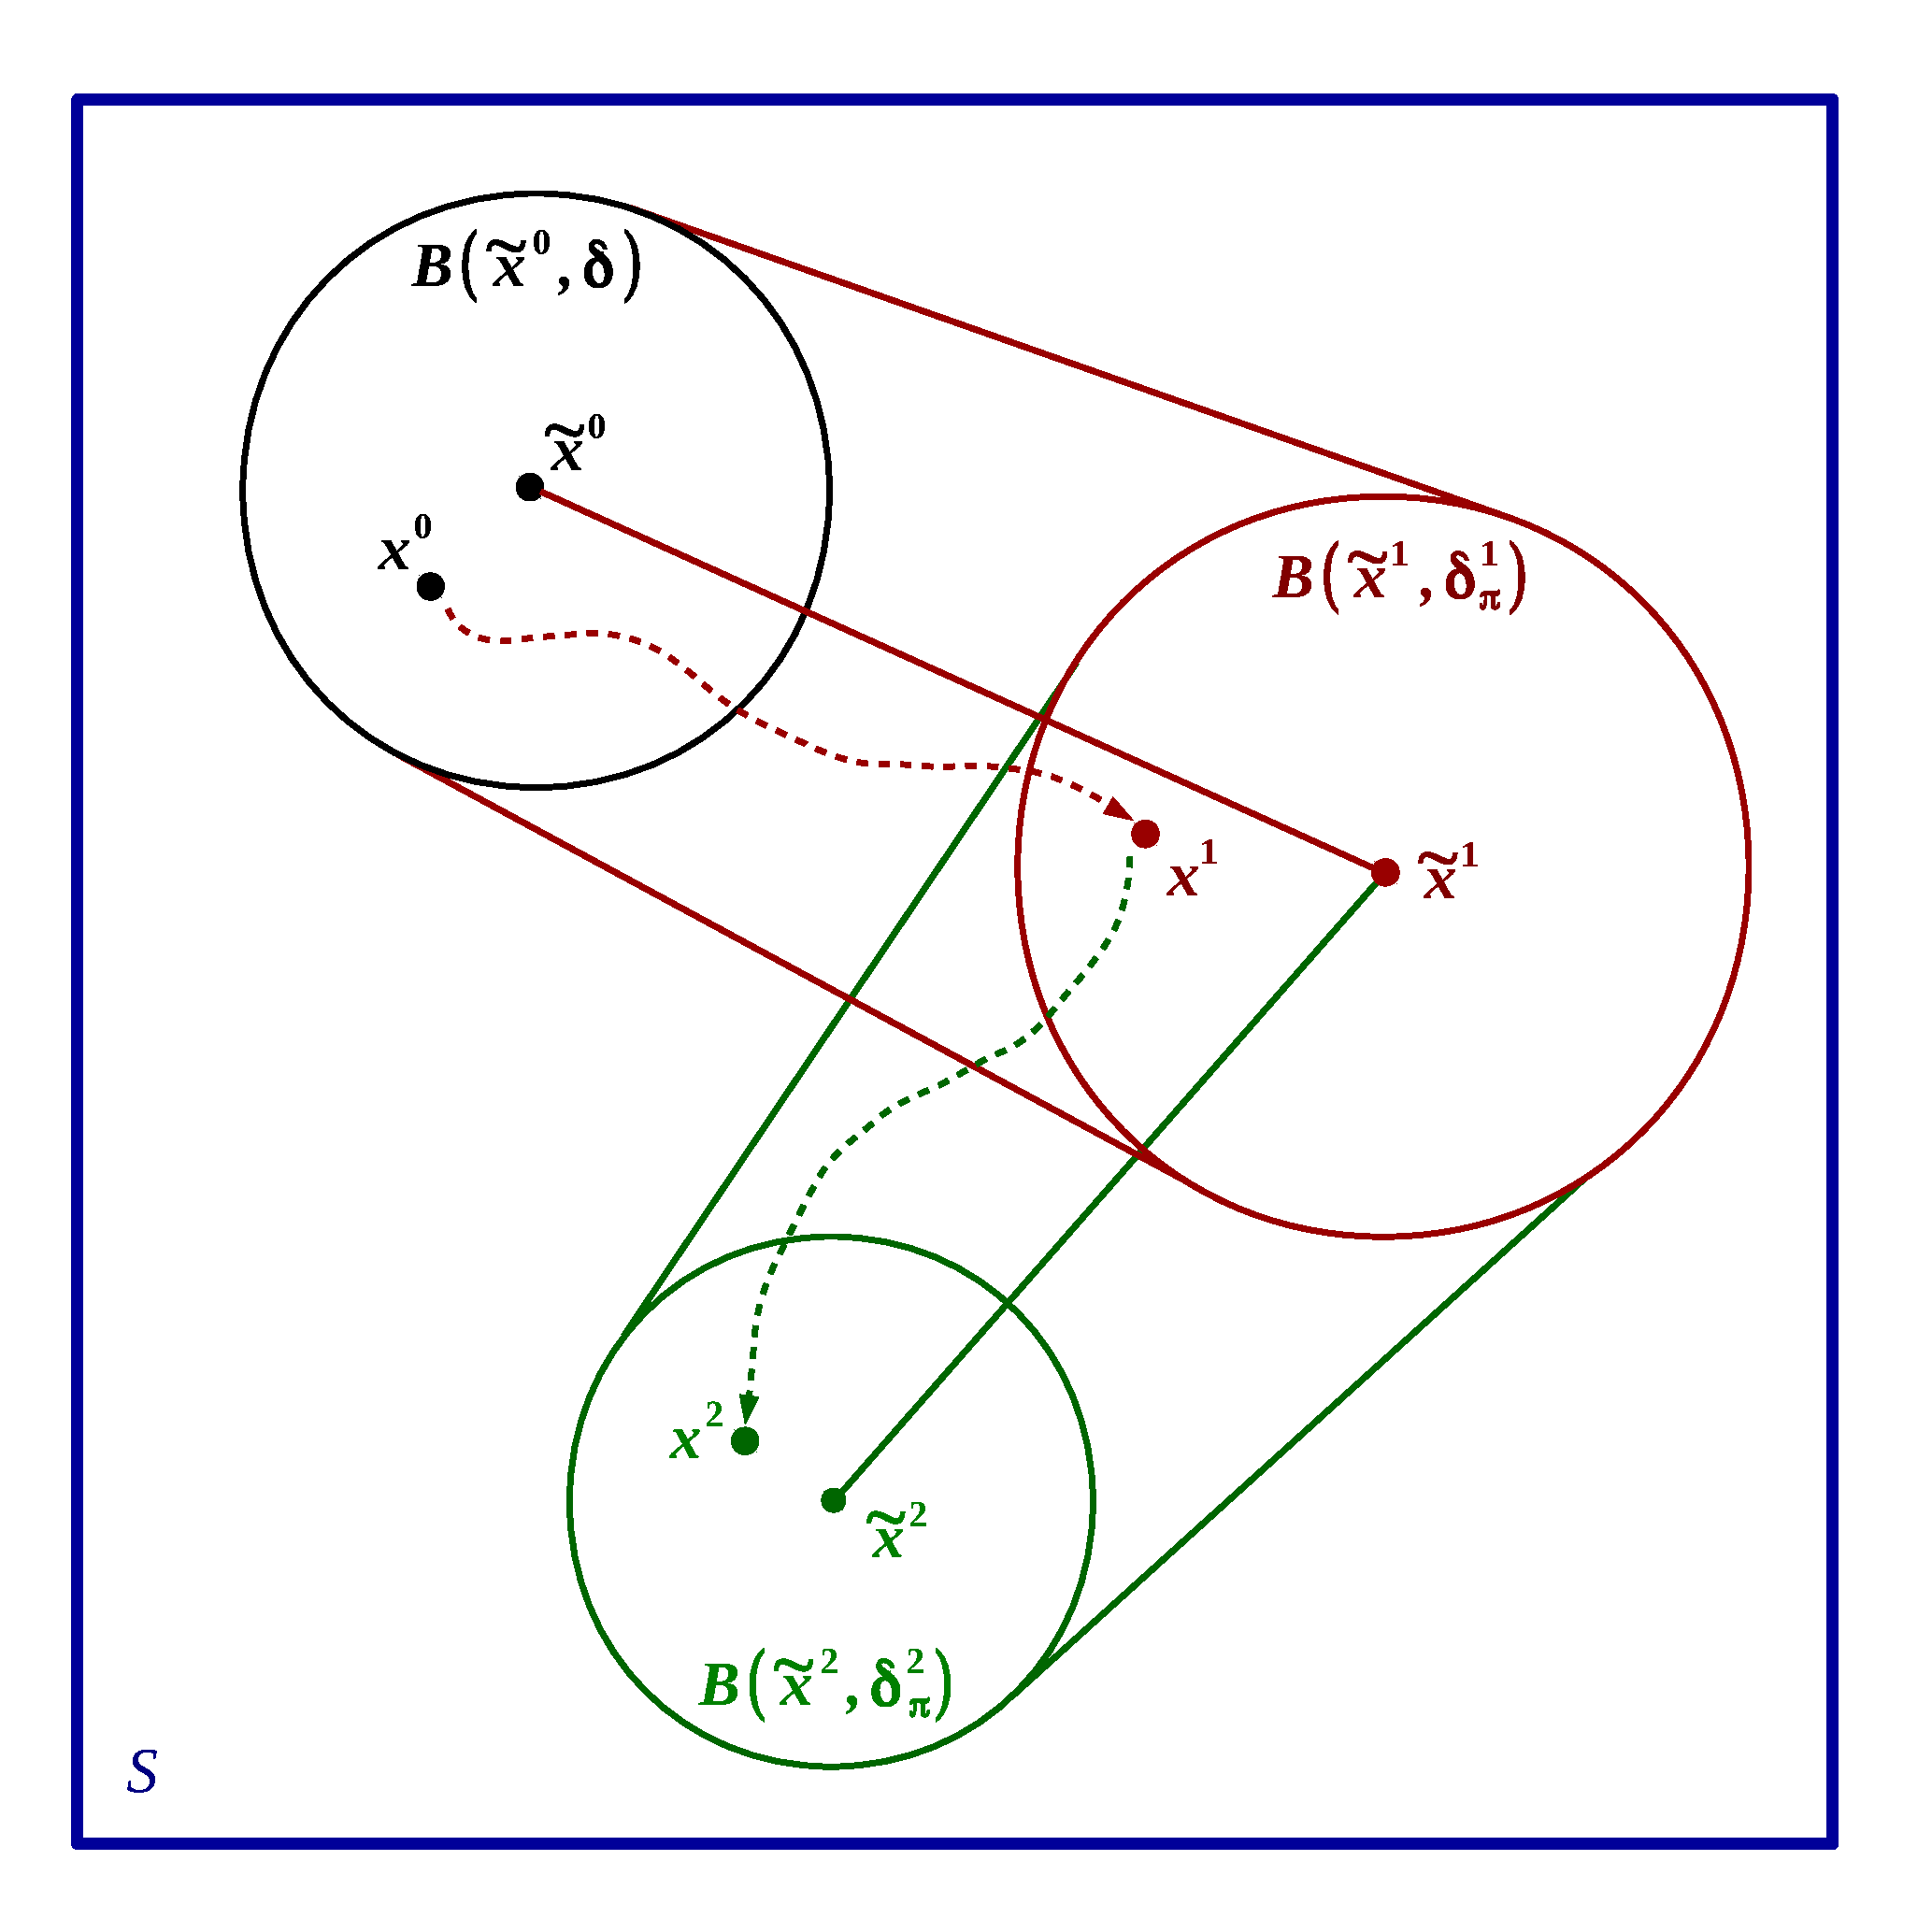
\includegraphics[width=0.4\linewidth,clip,trim=1cm 0cm 1cm 0cm]{ballimage.pdf}
\caption{Illustration of Theorem \ref{propbis:1}.}
%(with $\tilde y_0=\tilde \phi_\pi(\tau,\tilde x_0)$, $\tilde z_0=\tilde \phi_\pi(2\tau,\tilde x_0)$, $y_0=\phi_\pi(\tau,x_0)$, $z_0=\phi_\pi(2\tau,x_0))$.}
 \label{fig:tube}
\end{figure}



\begin{corollary}
Given a switched system satisfying (H0-H1), consider
%and an approximate  model \eqref{eq:sys_part22}. 
a positive real $\delta$ %with~$\delta\geq \frac{C_j\tau}{\lambda}$. 
%
and a finite set of points
$\tilde{x}_1,\dots\tilde{x}_m$ of $S$ such that all the balls $B(\tilde{x}_i,\delta)$ 
cover $R$ and are included into~$S$ (i.e. $R\subseteq \bigcup_{i=1}^mB(\tilde{x}_i,\delta)\subseteq S$).
%
Suppose furthermore that, for all $1\leq i\leq m$, there exists a pattern $\pi_i$ of length $k_i$ such that:
\begin{enumerate}
%\item $B(\tilde{\phi}_{\pi_i}(k'\tau;\tilde{x}_i), \delta_{\pi_i}(k'\tau)) \subseteq S$,
\item $B((\tilde{x}_i)_{\pi_i}^{k'},\delta_{\pi_i}^{k'}) \subseteq S$,
for all $k'=1,\dots,k_i-1$
%
\item 
%$B(\tilde{\phi}_{\pi_i}(k_i\tau;\tilde{x}_i), \delta_{\pi_i}(k_i\tau)) \subseteq R.$
$B((\tilde{x}_i)_{\pi_i}^{k_i}, \delta_{\pi_i}^{k_i}) \subseteq R.$
%
\item $\frac{d^2(\delta'_j(t))}{dt^2}>0$ 
with $j=\pi_i(k')$ and $\delta'=\delta_{\pi_i}^{k'-1}$, for all 
$k'\in\{1,...,k_i\}$ and $t\in [0,\tau]$.
%$\frac{d^2(\delta'_j(t)}{dt^2}>0$ for all $t\in [0,\tau]$, $j\in U$ and $\delta'\in [\delta]$.
\end{enumerate}
These properties induce a control
$\sigma$\footnote{Given an initial point $x\in R$, the induced control $\sigma$ corresponds to a sequence
of patterns $\pi_{i_1},\pi_{i_2},\dots$ defined as follows:
Since  $x\in R$, there exists a 
a point $\tilde{x}_{i_1}$  with $1\leq i_1\leq m$ such that $x\in B(\tilde{x}_{i_1},\delta)$; then using pattern $\pi_{i_1}$, one has: $\phi_{\pi_{i_1}}(k_{i_1}\tau;x)\in R$. Let $x'=\phi_{\pi_{i_1}}(k_{i_1}\tau;x)$; there exists a point $\tilde{x}_{i_2}$ with $1\leq i_2\leq m$ such that $x'\in B(\tilde{x}_{i_2},\delta)$, etc.}
%
which guarantees
%Let $k_{max}=\max_{i=1,\dots,m}\{k_i\}$.
\begin{itemize}
\item (safety): if $x\in R$, then $\phi_{\sigma}(t;x) \in S$ for all $t\geq 0$,
and
\item (recurrence):
if $x\in R$ then $\phi_{\sigma}(k\tau;x)\in R$ for some $k\in\{k_1,\dots,k_m\}$.
\end{itemize}
%
\label{propter:1}
\end{corollary}


Corollary \ref{propter:1} gives the theoretical foundations of the following method for synthesizing $\sigma$ ensuring recurrence in $R$ and safety in $S$:
\begin{itemize}
\item we (pre-)compute $\lambda_j, L_j, C_j$ for all $j\in U$;
\item we find $m$ points $\tilde{x}_1,\dots\tilde{x}_m$ of $S$
and $\delta>0$ such that $R\subseteq \bigcup_{i=1}^m B(\tilde{x}_i,\delta)\subseteq S$;
%for some $\delta>0$;%\geq \frac{C_j\tau}{\lambda}$;
\item we find $m$ patterns $\pi_i$  ($i=1,...,m$)
such that conditions 1-2-3 of Corollary \ref{propter:1} are satisfied.
\end{itemize} 
%
A covering of $R$ with balls as stated in Corollary \ref{propter:1} is illustrated in Figure \ref{fig:tiling}.
The control synthesis method based on~Corollary \ref{propter:1}
is illustrated in Figure \ref{fig:post} (left)
together with an illustration of method of \cite{NL_minimator} (right).

\begin{figure}[h]
\centering
 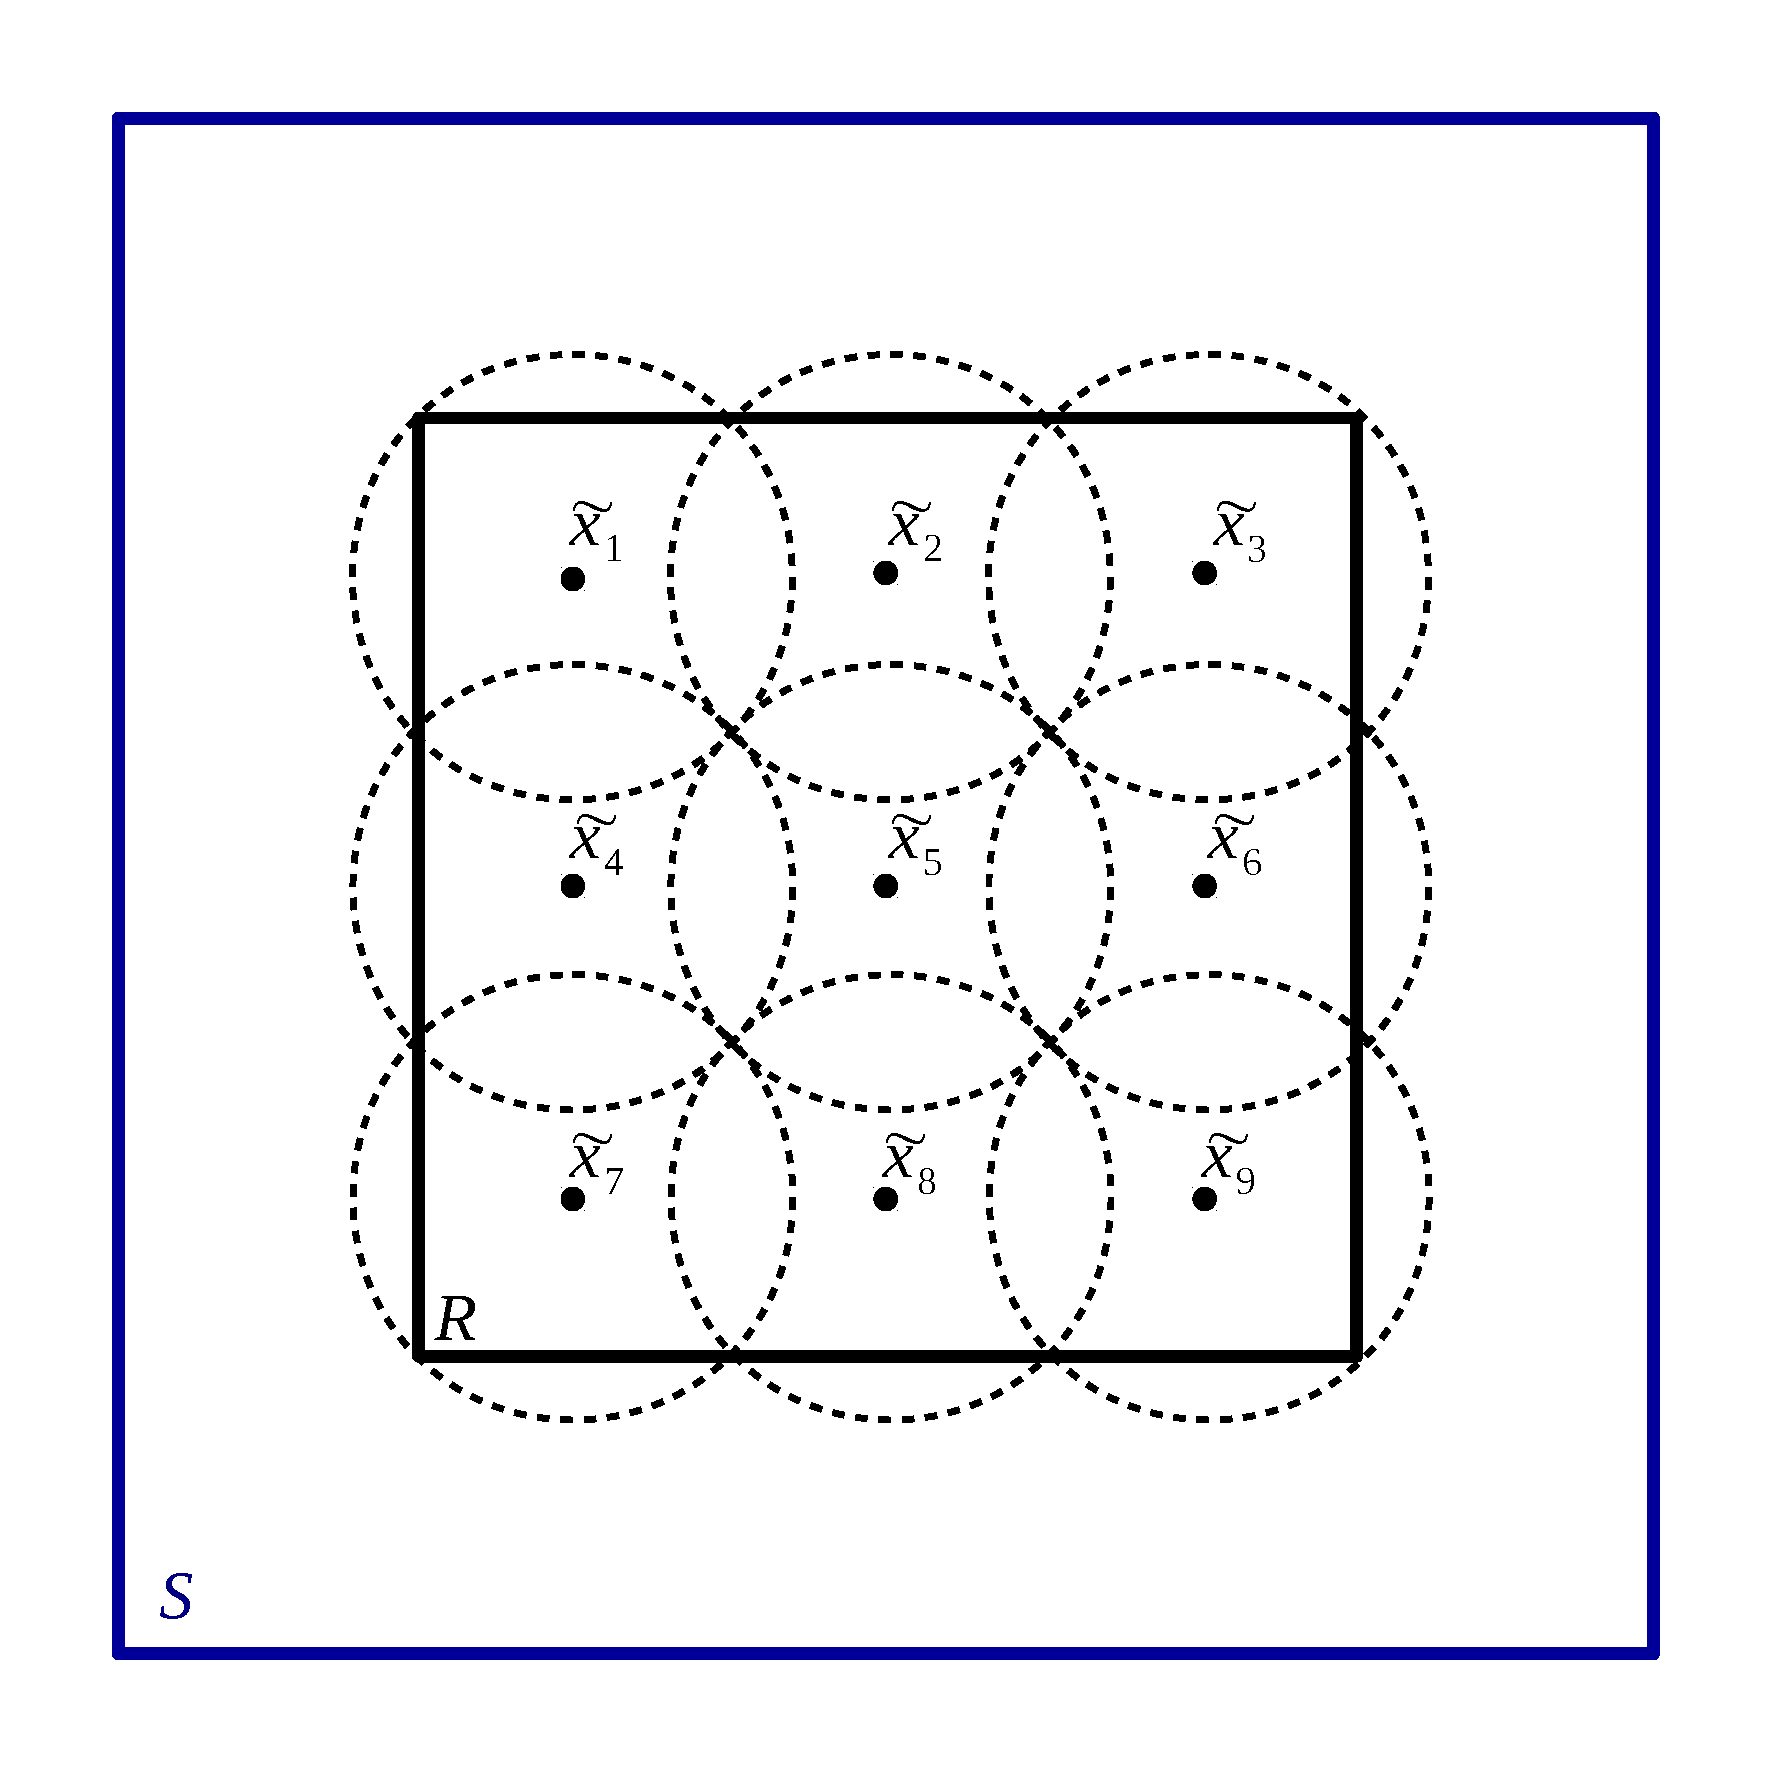
\includegraphics[width=0.4\linewidth,clip,trim=1cm 0cm 1cm 0cm]{tilingball2.pdf}
\caption{A set of balls covering $R$ and contained in $S$.}
\label{fig:tiling}
\end{figure}



%\begin{remark}
%en fait vrai pour tout $0\leq t\leq k\tau$ (et pas seulement $0\leq t<k\tau$).
%\end{remark}

\begin{figure}[h]
\centering
\begin{tabular}{cc}
 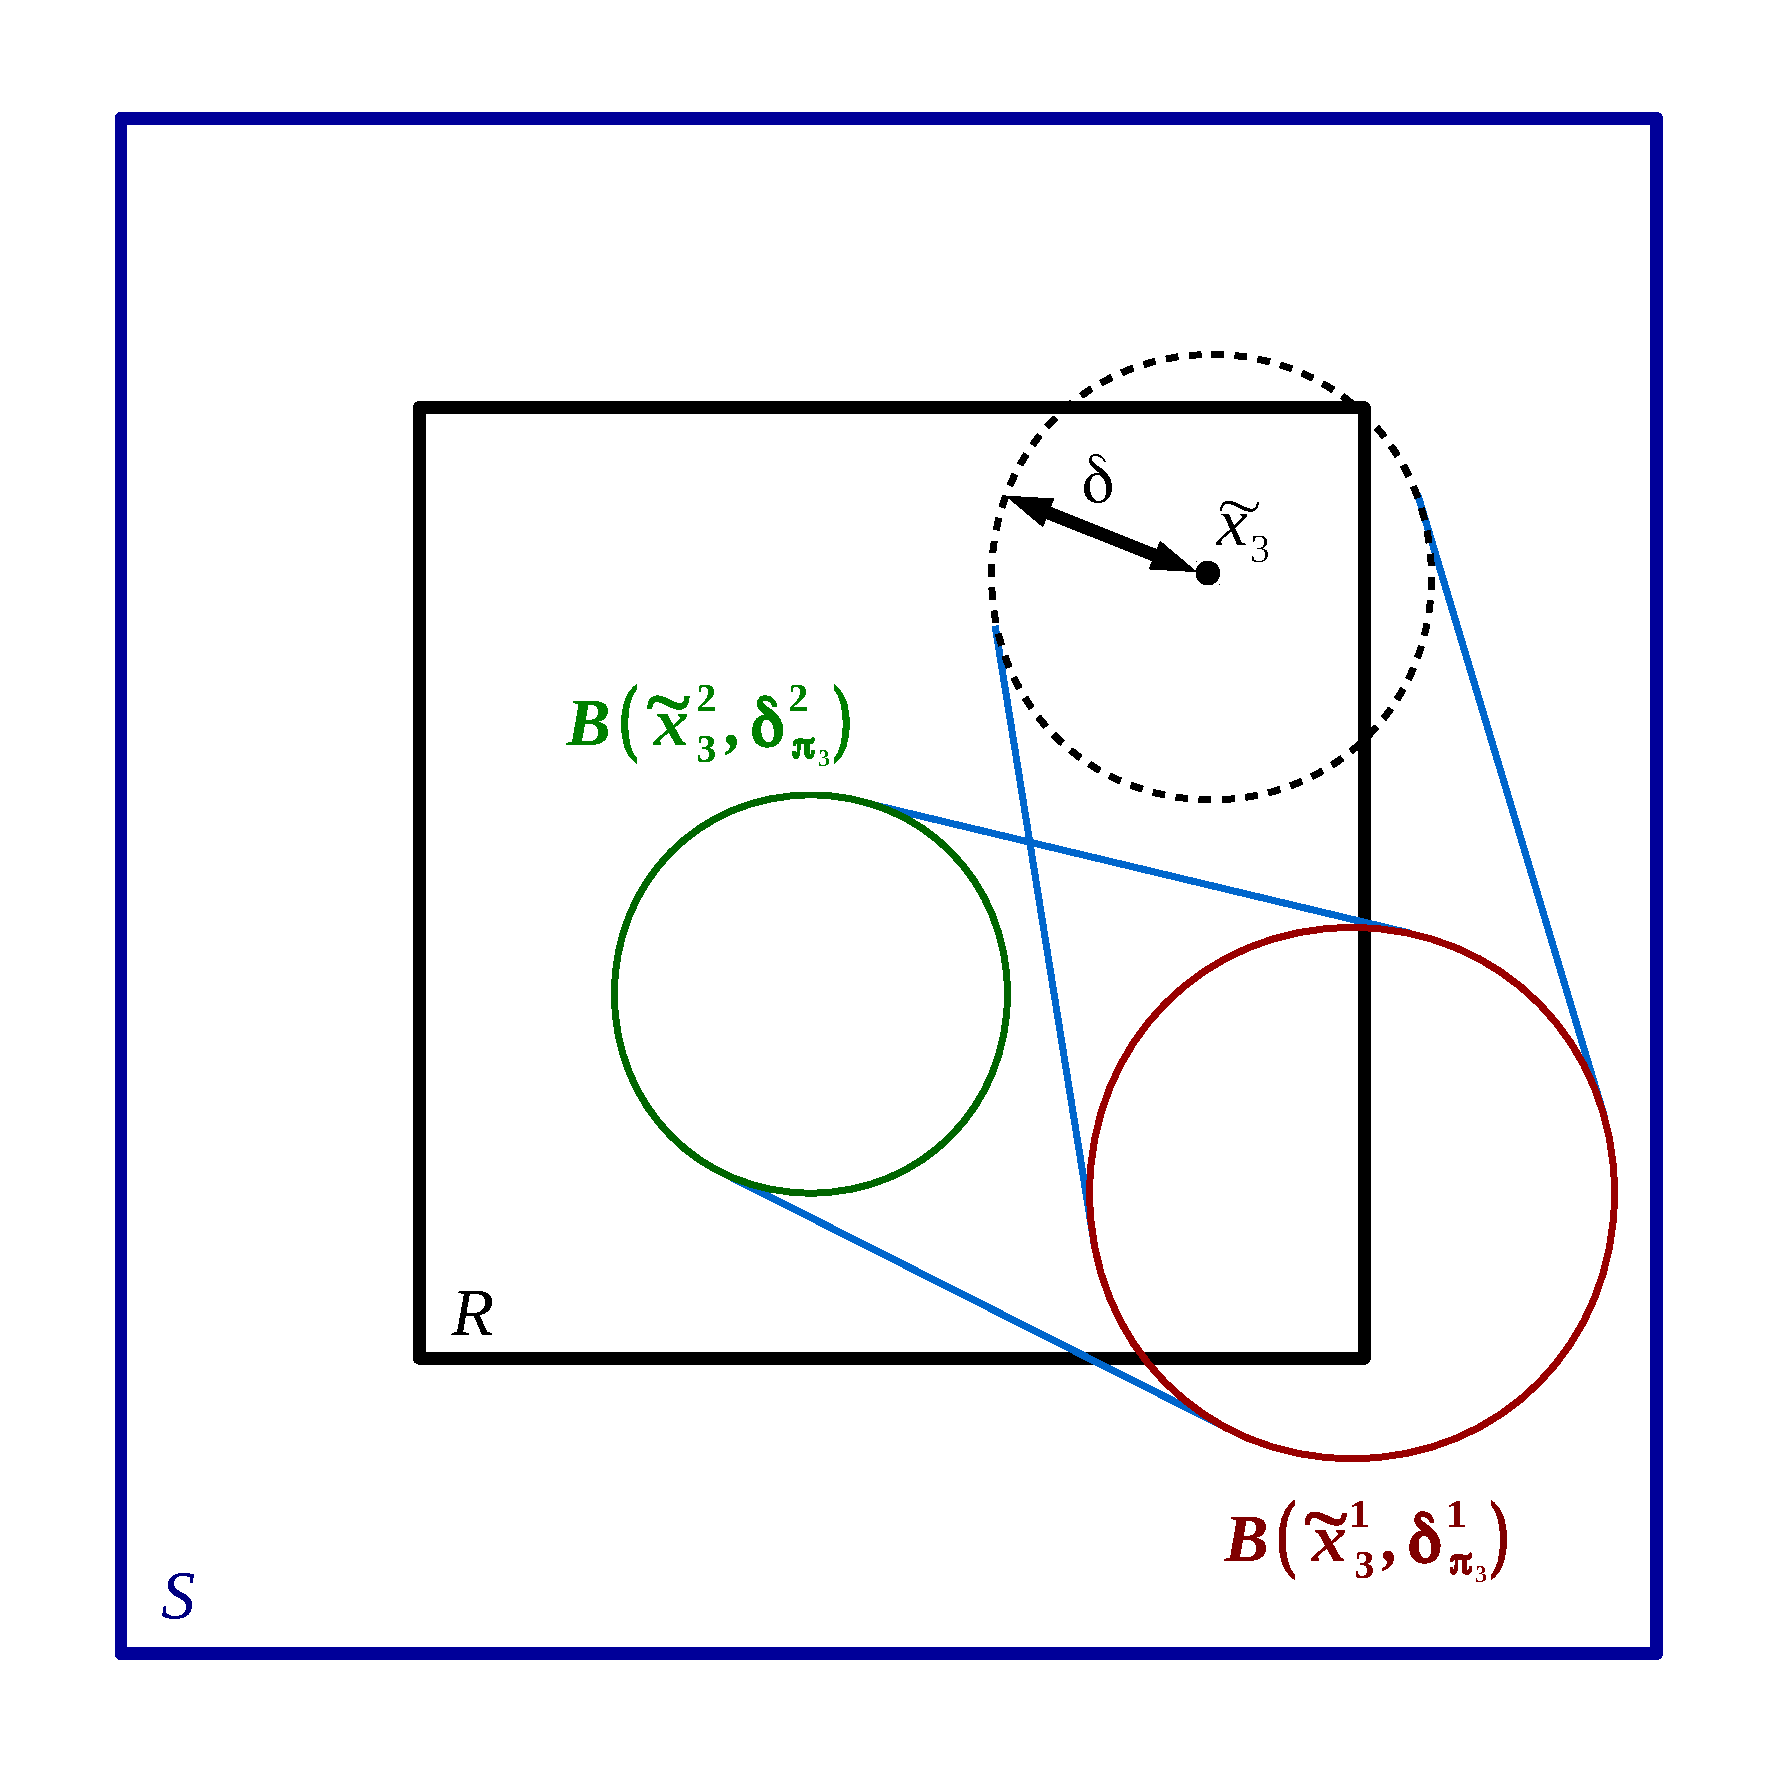
\includegraphics[width=0.4\linewidth,clip,trim=1cm 0cm 1cm 0cm]{tilingballimage.pdf}
&
 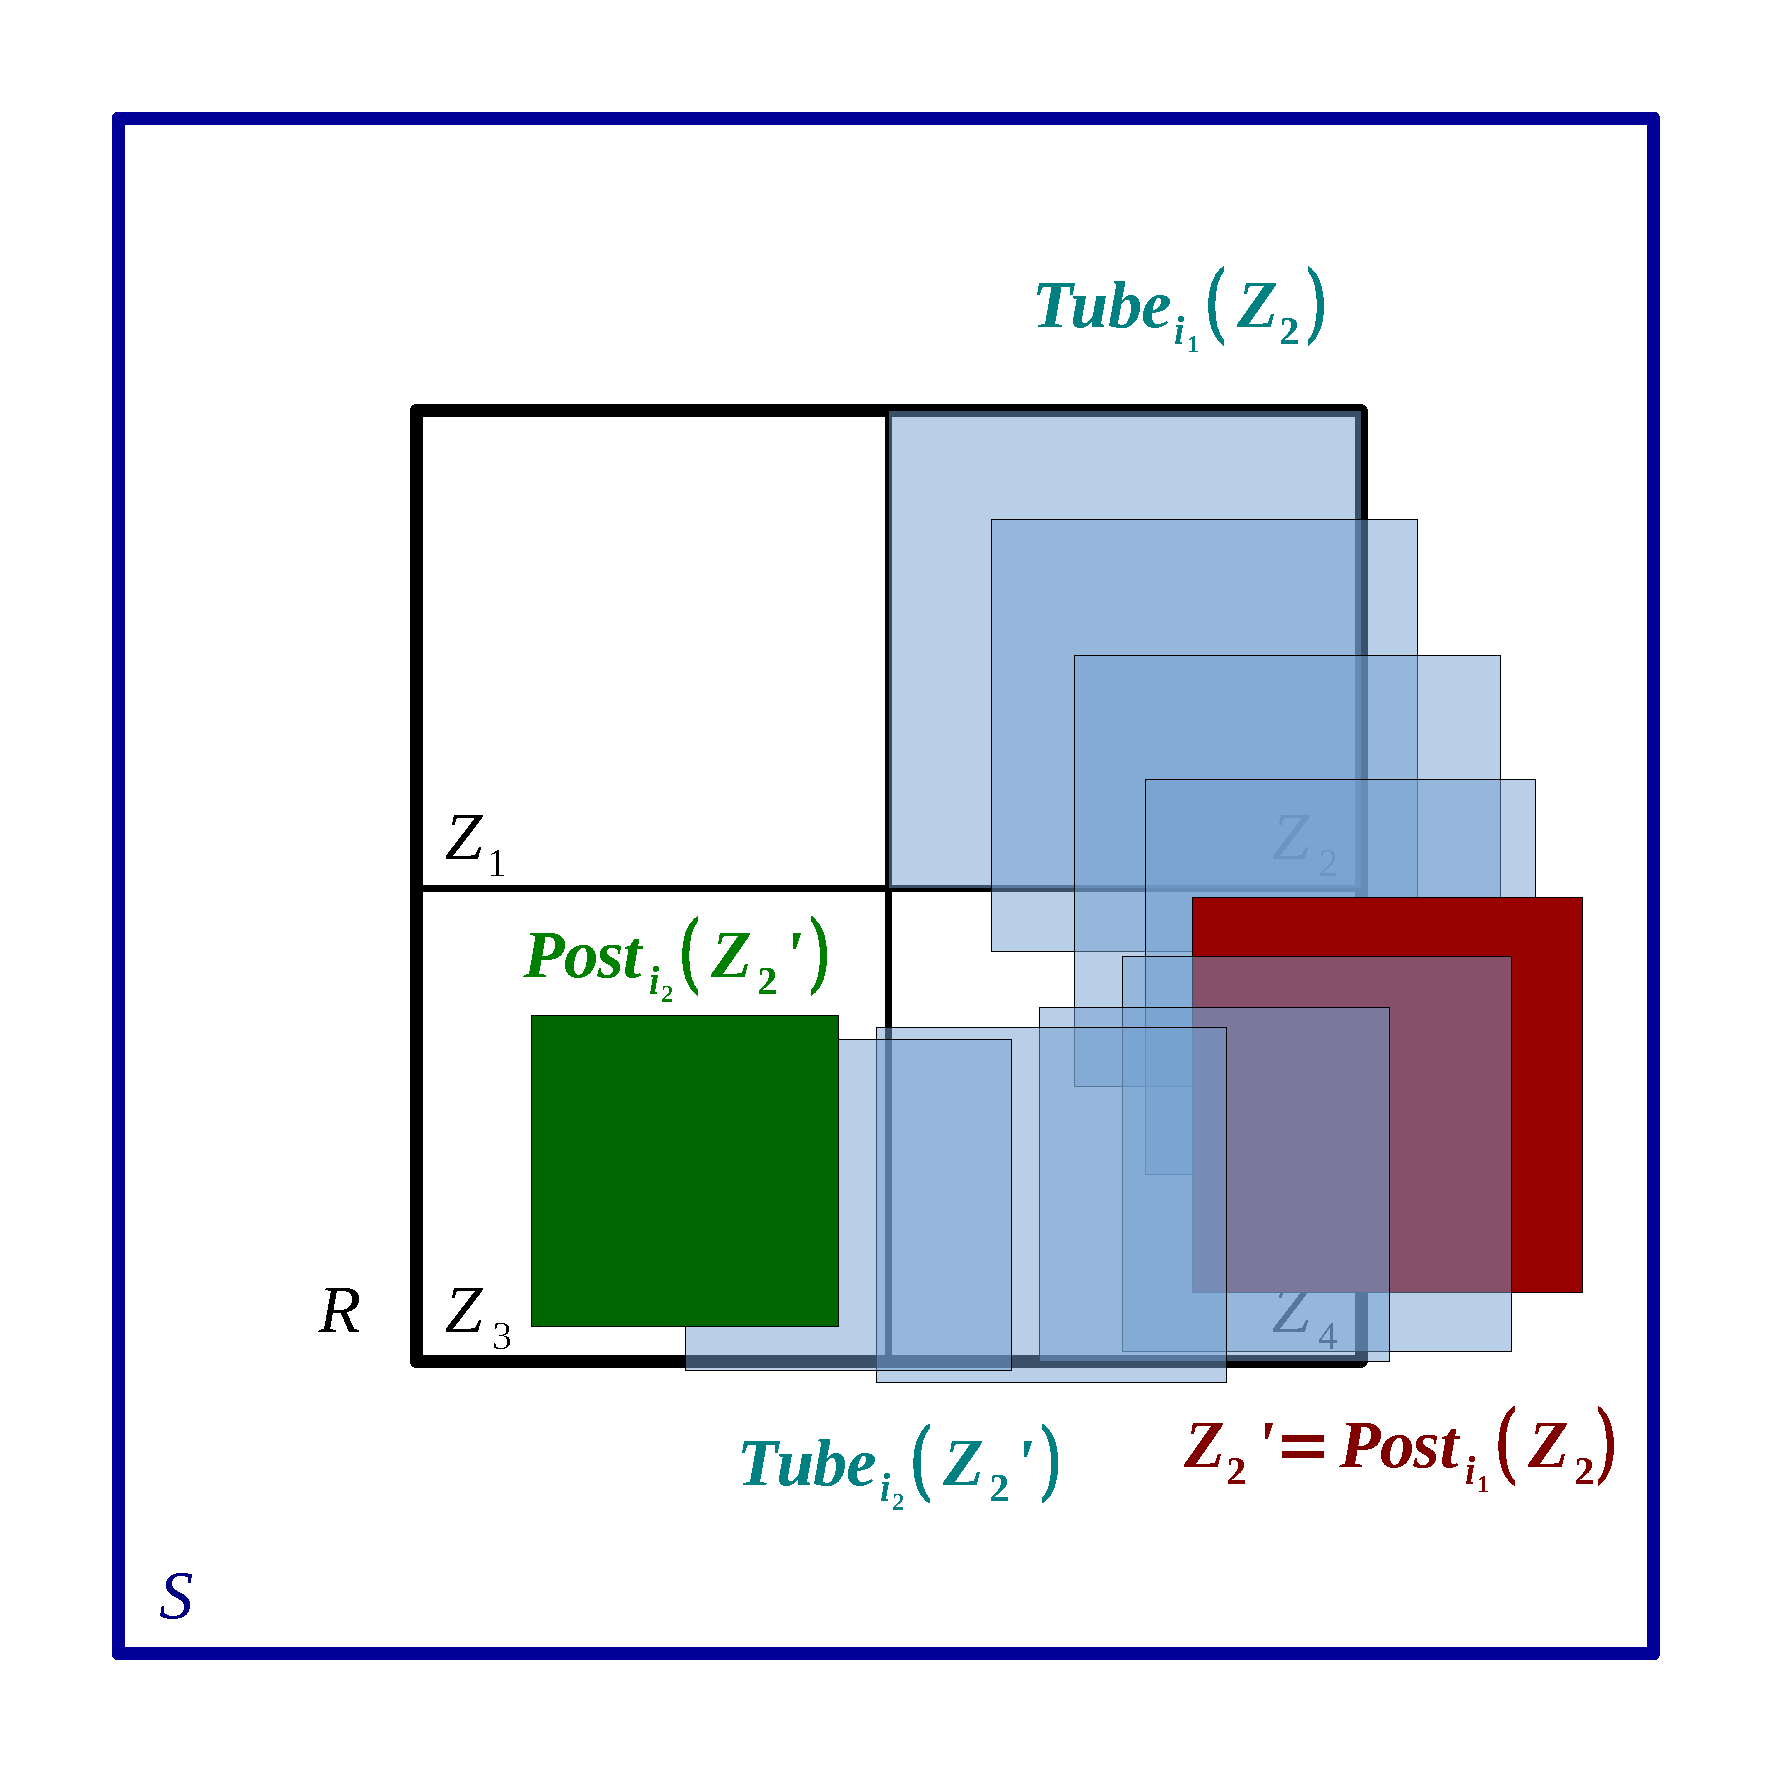
\includegraphics[width=0.4\linewidth,clip,trim=1cm 0cm 1cm 0cm]{snr16.pdf}
\end{tabular}
\caption{Control of ball $B(\tilde x_3,\delta)$ with our method (left);  
control of tile $Z_2$ with the method of \cite{NL_minimator}~(right).}
\label{fig:post}
\end{figure}


{\todo ??? Reformuler theoremes avec Post/Tube operators}




\subsection{Numerical experiments and results}
\label{sec:experiment}
This method has been implemented in the interpreted language Octave, 
and the experiments performed on a 2.80 GHz Intel Core i7-4810MQ CPU with 8 GB
of memory.



Note that in some cases, it is advantageous to use a time sub-sampling to compute the image of a ball.
Indeed, because of the exponential growth of the radius $\delta_j(t)$ within time,
computing a sequence of balls can lead to smaller ball images. 
It is particularly advantageous when a constant $\lambda_j$ is negative.
We illustrate this with the example of the DC-DC converter. 
It has two switched modes, for which we have $\lambda_1 = -0.014215$
and $\lambda_2 = 0.142474$. 
In the case $\lambda_j < 0$, the associated formula $\delta_j(t)$ has the behavior 
of Figure \ref{fig:delta_t_pos} (a). 
In the case $\lambda_j > 0$, the associated formula $\delta_j(t)$ has the behavior 
of Figure \ref{fig:delta_t_pos} (b). In the case $\lambda_j < 0$, 
if the time sub-sampling is small enough, 
one can compute a sequence of balls with reducing radius, which makes the synthesis easier. 

\begin{figure}[h]
\centering
\begin{tabular}{cc}
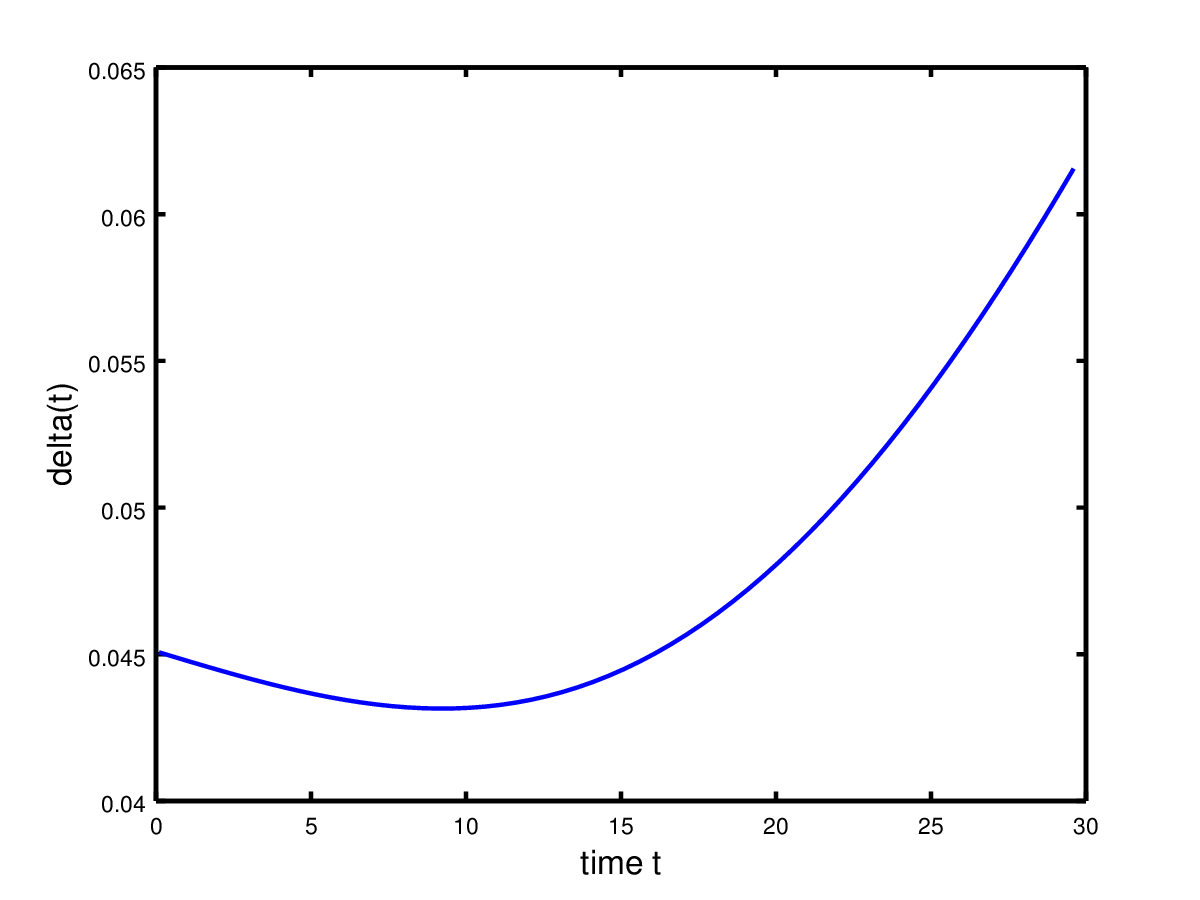
\includegraphics[width=0.45\linewidth,clip,trim=0.7cm 0cm 1.0cm 0cm]{deltatneg.png} & 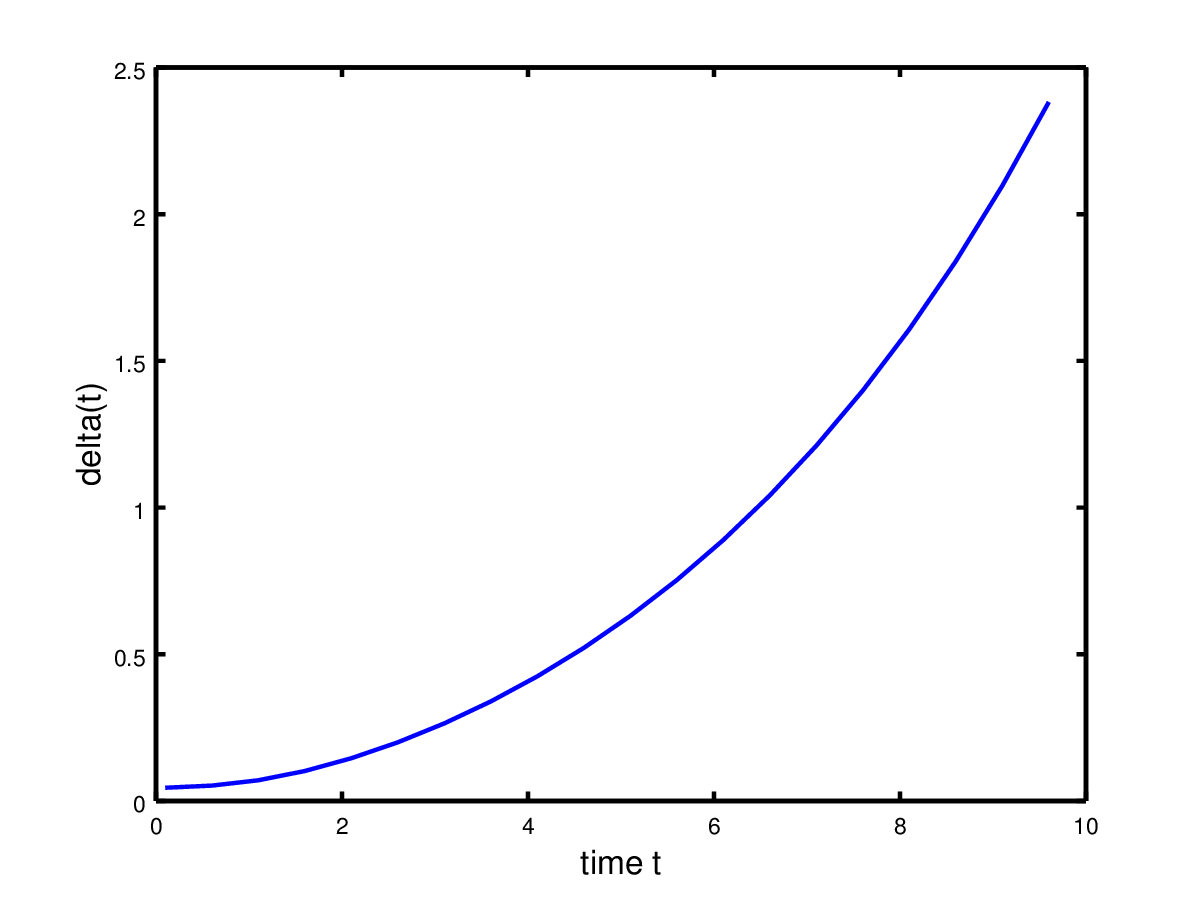
\includegraphics[width=0.45\linewidth,clip,trim=0.7cm 0cm 1.0cm 0cm]{deltatpos.png} \\
(a) & (b)
\end{tabular}
 \caption{Behavior of $\delta_j(t)$ for the DC-DC converter with $\delta_j(0) = 0.045$. 
 (a) Evolution of $\delta_1(t)$ (with $\lambda_1<0$); 
 (b) Evolution of $\delta_2(t)$ (with $\lambda_2>0$). }
  \label{fig:delta_t_pos}
 \end{figure}

In the following, we give the results obtained with our Octave implementation 
of this Euler-based method on 5 examples, and compare them with those 
given by the C++ implementation {\em DynIBEX} \cite{dynibex} of the Runge-Kutta based 
method used in \cite{NL_minimator}.


 \subsubsection{Four-room apartment}
 \label{sec:four_room}
 
 We describe a first application on a 4-room 16-switch building ventilation case study adapted from
\cite{meyer:tel-01232640}. The model has been simplified in order to get constant
parameters.
%, so that it can be handled by our linear tool MINIMATOR \cite{ulrich}, and
%a comparison can be performed with the C++ implementation presented in \cite{le2016control}
The system is a four room apartment
subject to heat transfer between the rooms, with the external
environment, the underfloor, and human beings.  The dynamics
of the system is given by the following equation:
\begin{equation*}
 \frac{d T_i}{dt} = \sum_{j \in \mathcal{N}^\text{*} \setminus \{i\}} a_{ij} (T_j -
 T_i) + \delta_{s_i} b_i (T_{s_i}^4 - T_i ^4 )  + c_i
 \max\left(0,\frac{V_i - V_i^\text{*}}{\bar{ V_i} -
   V_i^{\text{*}}}\right)(T_u - T_i), \quad \mbox{for } i=1,...,4.
\end{equation*}

The state of the system is given by the temperatures in the rooms
$T_i$, for $i \in \mathcal{N} = \{ 1 , \dots , 4 \}$.  Room~$i$ is
subject to heat exchange with different entities stated by the indices
$\mathcal{N}^\text{*} = \{1,2,3,4,u,o,c \}$.
%
We have $T_0=30, T_c=30, T_u=17$, $\delta_{s_i}=1$ for $i\in\mathcal{N}$.
The (constant) parameters $T_{s_i}$, $V_i^\text{*}$, $\bar V_i$, $a_{ij}$, $b_i$,
$c_i$ are given in~\cite{meyer:tel-01232640}. 
%and have been identified
%with a proper identification procedure detailed in
%\cite{meyer2014ecc}. 
%Note that we have neglected the term $\sum_{j
%  \in \mathcal{N}} \delta_{d_{ij}}c_{i,j} \ast h(T_j - T_i)$ of
%\cite{meyer:tel-01232640},
%representing the perturbation induced by
%the open or closed state of the doors between the rooms.\\
%
The control input is $V_i$ ($i \in \mathcal{N}$).
%, is applied through the term
%$c_i \max(0,\frac{V_i - V_i^\text{*}}{\bar{ V_i} -
%  V_i^{\text{*}}})(T_u - T_i)$.  
%A voltage $V_i$ is applied to force
%ventilation from the underfloor to room $i$, and the command of an
%underfloor fan is subject to a dry friction.  Because we work in a
%switched control framework, $V_i$ can take only discrete values, which
%removes the problem of dealing with a ``max'' function in interval
%analysis. 
In the experiment, $V_1$ and $V_4$ can take the values $0$V
or $3.5$V, and $V_2$ and~$V_3$ can take the values $0$V or $3$V. This
leads to a system of the form~\eqref{eq:sys_part2} with $\sigma(t) \in U =\{
1, \dots, 16 \}$, the $16$ switching modes corresponding to the
different possible combinations of voltages $V_i$.  
The sampling period is $\tau = 30$s.
Compared simulations are given in Figure \ref{fig:simu}.
On this example, the Euler-based method works better than {\em DynIBEX}
in terms of CPU time.



 \begin{table}[h]
 \centering
\begin{tabular}{|c|c|c|}
   \hline 
   &\multicolumn{1}{c|}{Euler} & \multicolumn{1}{c|}{DynIBEX} \\
   \hline
   $R$ & \multicolumn{2}{c|}{$[20,22]^2\times[22,24]^2$} \\
   $S$ & \multicolumn{2}{c|}{$[19,23]^2\times[21,25]^2$} \\   
\hline
$\tau$ & \multicolumn{2}{c|}{30} \\
\hline
Time subsampling & No & \\   
   \hline
 Complete control & Yes  & Yes \\
\hline
$\max_{j= 1, \dots,16} \lambda_j$  &  $-6.30\times 10^{-3}$   &        \\
$\max_{j= 1, \dots,16} C_j$  &  $4.18\times 10^{-6}$ &                     \\
\hline
Number of balls/tiles & 4096 & 252 \\
Pattern length & 1 & 1 \\
\hline
CPU time &  63 seconds & 249 seconds\\ \hline
  \end{tabular}
\label{table:4M}
\caption{Numerical results for the four-room example.}
 \end{table} 
 

\begin{figure}[h]
\centering
\begin{tabular}{cc}
% 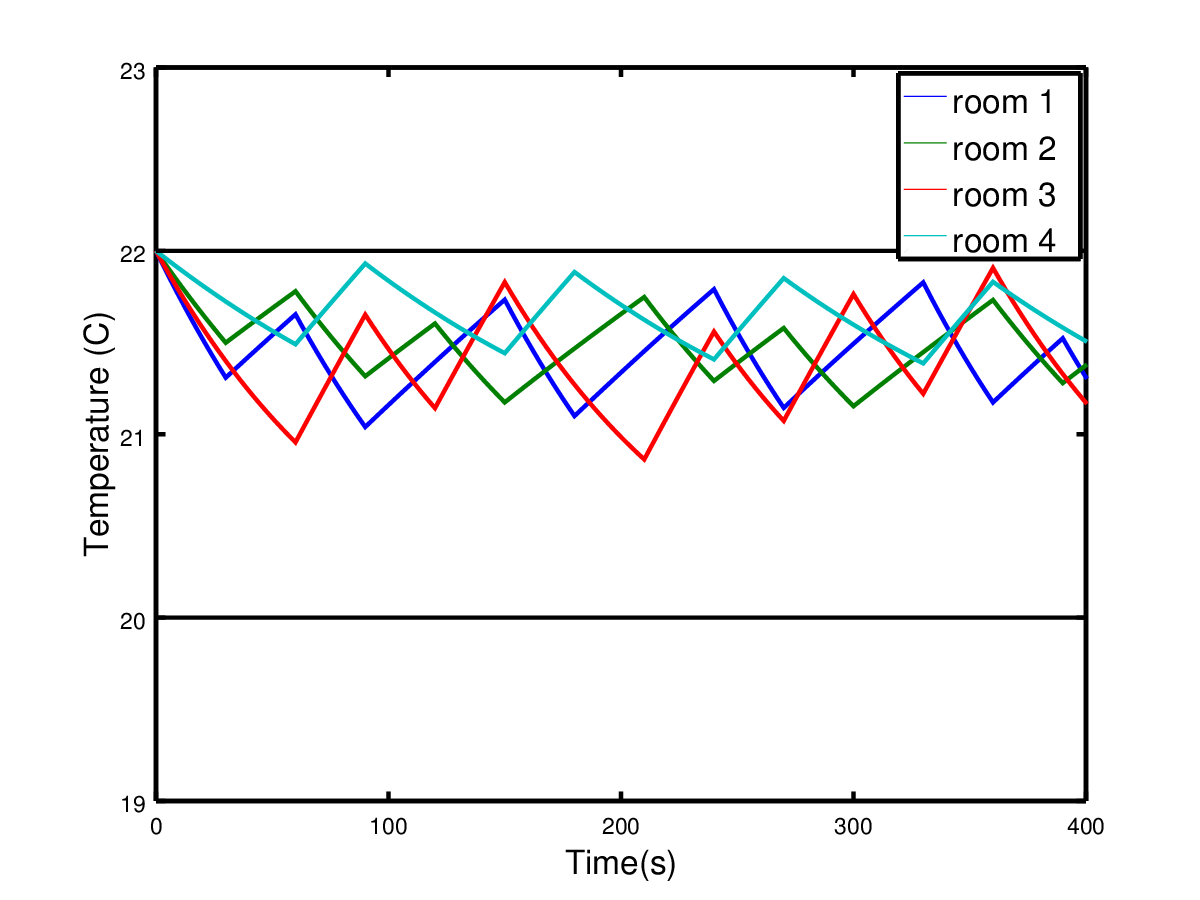
\includegraphics[width=0.45\linewidth,clip,trim=1cm 0cm 1cm 0cm]{simu4rooms3linear.png}
 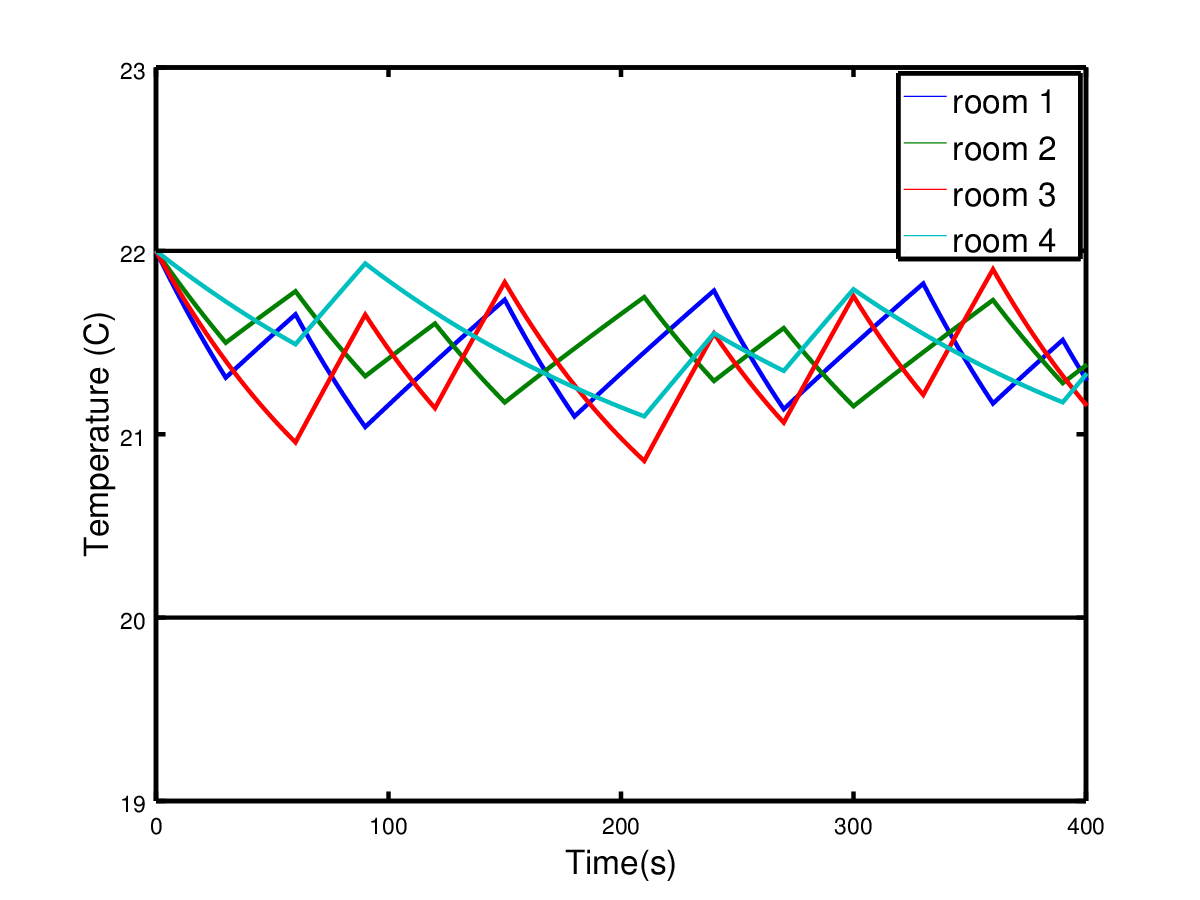
\includegraphics[width=0.4\linewidth,clip,trim=1cm 0cm 1cm 0cm]{simu4roomslinearnew.png}
&
 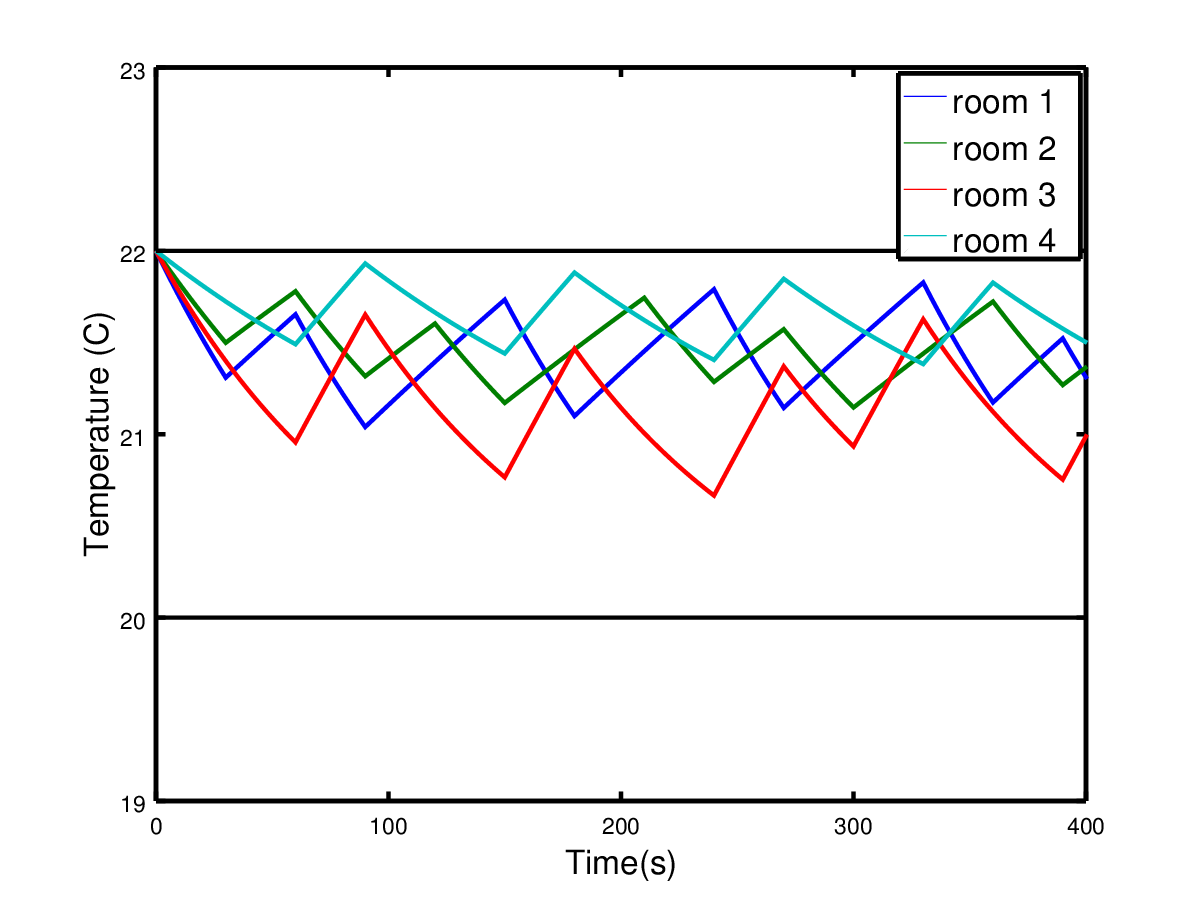
\includegraphics[width=0.4\linewidth,clip,trim=1cm 0cm 1cm 0cm]{simu4rooms2.png}
\end{tabular}
\caption{Simulation of the four-room case study with our synthesis method (left) and with the synthesis method of \cite{NL_minimator}  (right).}
\label{fig:simu}
\end{figure}

\subsubsection{DC-DC converter}

This linear example is taken from \cite{beccuti2005optimal} and has
already been treated with the state-space bisection method in a linear
framework in \cite{fribourg2014finite}.

The system is a boost DC-DC converter with one switching cell.  There
are two switching modes depending on the position of the switching
cell. The dynamics is given by the equation $\dot x (t) =
A_{\sigma(t)} x(t) + B_{\sigma(t)}$ with $\sigma(t) \in U = \{ 1,2
\}$. The two modes are given by the matrices:

$$ A_1 = \left( \begin{matrix}
          - \frac{r_l}{x_l} & 0 \\ 0 & - \frac{1}{x_c} \frac{1}{r_0 + r_c}
         \end{matrix} \right)  \quad B_1 = \left( \begin{matrix}
         \frac{v_s}{x_l} \\ 0 \end{matrix} \right) $$


$$ A_2 = \left( \begin{matrix} - \frac{1}{x_l} (r_l +
  \frac{r_0.r_c}{r_0 + r_c}) & - \frac{1}{x_l} \frac{r_0}{r_0 + r_c}
  \\ \frac{1}{x_c}\frac{r_0}{r_0 + r_c} & - \frac{1}{x_c}
  \frac{r_0}{r_0 + r_c}
         \end{matrix} \right)  \quad B_2 = \left( \begin{matrix}
         \frac{v_s}{x_l} \\ 0 \end{matrix} \right)  $$

with $x_c = 70$, $x_l = 3$, $r_c = 0.005$, $r_l = 0.05$, $r_0 = 1$,
$v_s = 1$.  The sampling period is $\tau = 0.5$.  The parameters are
exact and there is no perturbation.  We want the state to return
infinitely often to the region~$R$, set here to $\lbrack 1.55 , 2.15
\rbrack \times \lbrack 1.0 , 1.4 \rbrack$, while never going out of
the safety set $S = \lbrack 1.54 , 2.16 \rbrack \times \lbrack 0.99 ,
1.41 \rbrack$.
%
On this example, the Euler-based method {\em fails} while {\em DynIBEX} succeeds
rapidly.


\begin{table}[h]
 \centering
\begin{tabular}{|c|c|c|}
\hline 
 &\multicolumn{1}{c|}{Euler} & \multicolumn{1}{c|}{DynIBEX} \\
\hline
$R$ & \multicolumn{2}{c|}{$[1.55,2.15]\times[1.0,1.4]$} \\
$S$ & \multicolumn{2}{c|}{$[1.54,2.16]\times[0.99,1.41]$} \\
\hline
$\tau$ &\multicolumn{2}{c|}{ 0.5 }\\
\hline
 Complete control & No & Yes\\
\hline
$\lambda_1$  & $-0.014215$ &\\
$\lambda_2$  & $0.142474$ &\\
$C_{1}$  & $6.7126 \times 10^{-5}$ &\\
$C_{2}$ &  $2.6229 \times 10^{-2}$ &\\
\hline
Number of balls/tiles & x & 48 \\
\hline
Pattern length & x & 6 \\
\hline
CPU time & x & < 1 second \\ \hline
 \end{tabular}
\label{table:DC}
\caption{Numerical results for the DC-DC converter example.}
 \end{table}



 \subsubsection{Polynomial example}
 We consider the polynomial system taken from \cite{liu2013synthesis}:
%
\begin{equation}
 \left \lbrack \begin{matrix}
  \dot x_1 \\ \dot x_2
 \end{matrix} \right \rbrack  =
 \left \lbrack \begin{matrix} -x_2 - 1.5 x_1 - 0.5 x_1^3 + u_1 \\ x_1 + u_2 
   \end{matrix} \right \rbrack.
\end{equation}
%
The control inputs are given by $u = (u_1,u_2) =
K_{\sigma(t)}(x_1,x_2)$, $\sigma(t) \in U = \{ 1,2,3,4 \}$, which correspond to
four different state feedback controllers $K_1(x) = (0,-x_2^2 + 2)$,
$K_2(x) = (0,-x_2)$, $K_3(x) = (2,10)$, $K_4(x) = (-1.5,10)$.  We thus
have four switching modes. The disturbances are not taken into account.
The objective is to visit infinitely often {\em two} zones $R_1$ and $R_2$,
without going out of a safety zone $S$.
 
 
 
 \begin{table}[ht]
 \centering
\begin{tabular}{|c|c|c|}
 \hline 
 &\multicolumn{1}{c|}{Euler} & \multicolumn{1}{c|}{DynIBEX} \\
\hline
 $R_1$ & \multicolumn{2}{c|}{$[-1,0.65]\times[0.75,1.75]$} \\
 $R_2$ & \multicolumn{2}{c|}{$[-0.5,0.5]\times[-0.75,0.0]$ }\\
 $S$ &  \multicolumn{2}{c|}{$[-2.0,2.0]\times[-1.5,3.0]$ }\\
 \hline
$\tau$ & \multicolumn{2}{c|}{0.15} \\
\hline
Time subsampling & $\tau/20$ & \\
\hline
 Complete control & Yes & Yes \\
\hline
$\lambda_1$  & $-1.5$   &   \\
$\lambda_2$  &  $-1.0$ &\\
$\lambda_3$  &  $-1.1992 \times 10^{-8}$ & \\
$\lambda_4$ &  $-5.7336 \times 10^{-6}$ & \\
$C_{1}$  &  641.37     &    \\
$C_{2}$ &  138.49 &\\
$C_{3}$  &  204.50 & \\
$C_{4}$ & 198.64 &\\
\hline
Number of balls/tiles & 16 \& 16 & 1 \& 1 \\
Pattern length & 8  & 7  \\
\hline
CPU time & 29 \& 4203  seconds & <0.1 \& 329 seconds \\ \hline
  \end{tabular}
\label{table:PE}
\caption{Numerical results for the polynomial example example.}
 \end{table}

For Euler and {\em DynIBEX}, the table indicates {\em two} CPU times corresponding to the reachability from $R_1$
to $R_2$ and vice versa.
On this example, the Euler-based method is much slower than {\em DynIBEX}.
 
 \subsubsection{Two-tank system}
 \label{sec:two_tank}
 
 The two-tank  system  is a linear example taken from \cite{hiskens2001stability}. The system consists of two tanks and two valves.
 The first valve adds to the inflow of tank 1 and the second valve is a drain valve for tank 2. 
 There is also a constant outflow from tank 2 caused by a pump. The system is linearized at a desired
 operating point. The objective is to keep the water level in both tanks 
 within limits using a discrete open/close switching strategy for the valves. 
 Let the water level of tanks 1 and 2 be given by $x_1$ and $x_2$ respectively. 
 The behavior of $x_1$ is given by $\dot x_1 = -x_1 - 2$ when the tank 1 valve is closed, 
 and $\dot x_1 = -x_1 + 3$ when it is open. Likewise,
 $x_2$ is driven by $\dot x_2 = x_1$ when the tank 2 valve is closed and $\dot x_2 = x_1 - x_2 - 5$ when it 
 is open. 
On this example, the Euler-based method works better than {\em DynIBEX}
in terms of CPU time.

 
 
 \begin{table}[ht]
 \centering
\begin{tabular}{|c|c|c|}
 \hline 
 &\multicolumn{1}{c|}{Euler} & \multicolumn{1}{c|}{DynIBEX} \\
\hline
$R$ & \multicolumn{2}{c|}{$[-1.5,2.5]\times[-0.5,1.5]$} \\
$S$ & \multicolumn{2}{c|}{$[-3,3]\times[-3,3]$} \\
\hline
$\tau$ & \multicolumn{2}{c|}{0.2} \\
\hline
Time subsampling & $\tau/10$ & \\
\hline
Complete control & Yes & Yes \\
\hline
$\lambda_1$  & 0.20711     &       \\
$\lambda_2$  &  -0.50000 &\\
$\lambda_3$  &  0.20711 &  \\
$\lambda_4$ &  -0.50000 & \\
$C_{1}$  &  11.662    &             \\
$C_{2}$ & 28.917&\\
$C_{3}$  &  13.416 &\\
$C_{4}$ & 32.804& \\
\hline
Number of balls/tiles & 64 & 10 \\
Pattern length & 6 & 6 \\
\hline
CPU time & 58 seconds & 246 seconds\\ \hline
  \end{tabular}
\label{table:TT}
\caption{Numerical results for the two-tank example.}
 \end{table}
 

 \subsubsection{Helicopter}
 \label{sec:helico}
 
 The helicopter is a linear example taken from \cite{ding2011reachability}. The problem is to control a quadrotor helicopter toward 
 a particular position on top of a stationary ground vehicle, while satisfying constraints 
 on the relative velocity. 
%By controlling the pitch and roll angles, we can modify the speed and the
% position of the helicopter. A typical problem is 
% to find a switching rule, depending on the position and velocity of 
% the helicopter, in order to keep the system 
% state within a safe area, avoiding excessive speed or distance in 
% relation to the ground vehicle. 
Let $g$ 
 be the gravitational constant, $x$ (reps. $y$) the position 
 according to $x$-axis (resp. $y$-axis), $\dot x$ (resp. $\dot y$) the velocity according to $x$-axis (resp. $y$-axis),
 $\phi$ the pitch command and $\psi$ the roll command. 
 The possible commands for the pitch and the roll are 
 the following: $\phi,\psi \in \{ -10,0,10 \}$.
 Since each mode corresponds to a pair $(\phi,\psi)$, there are nine switched modes.
 The dynamics of the system is given by the equation:
 $$ \dot X = \begin{pmatrix}
              0 & 1 & 0 & 0 \\ 
              0 & 0 & 0 & 0 \\ 
              0 & 0 & 0 & 1 \\               
              0 & 0 & 0 & 0               
              \end{pmatrix} X + \begin{pmatrix}
              0 \\ g\sin(-\phi) \\ 0 \\ g\sin(\psi) \end{pmatrix}              
 $$
where $X = ( x \ \dot x \ y \ \dot y)^\top$. Since the variables $x$ and $y$
are decoupled in the equations and follow the same equations (up to the sign of the command), it suffices
to study the control for $x$ (the control for $y$ is the opposite).
On this example again, the Euler-based method works better than {\em DynIBEX}
in terms of CPU time.

 \begin{table}[ht]
 \centering
\begin{tabular}{|c|c|c|}
   \hline 
   &\multicolumn{1}{c|}{Euler} & \multicolumn{1}{c|}{DynIBEX} \\
   \hline
   $R$ & \multicolumn{2}{c|}{$[-0.3,0.3]\times[-0.5,0.5]$} \\
   $S$ & \multicolumn{2}{c|}{$[-0.4,0.4]\times[-0.7,0.7]$} \\   
\hline
$\tau$ & \multicolumn{2}{c|}{0.1} \\
\hline
Time subsampling & $\tau/10$ & \\   
   \hline
 Complete control & Yes  & Yes \\
\hline
$\lambda_1$  & 0.5    &        \\
$\lambda_2$  &  0.5 &\\
$\lambda_3$  &  0.5 &  \\
$C_{1}$  &  1.77535 &                     \\
$C_{2}$ & 0.5 &\\
$C_{3}$  &   1.77535& \\
\hline
Number of balls/tiles & 256 & 35 \\
Pattern length & 7 & 7 \\
\hline
CPU time &  539 seconds & 1412 seconds\\ \hline
  \end{tabular}
\label{table:HM}
\caption{Numerical results for the helicopter motion example.}
 \end{table} 

 

\subsubsection{Analysis and comparison of results}


This method presents a great advantage over the recent work~\cite{le2016control}:
no numerical integration is required for the control synthesis. 
% It does not require any inversion of matrices (such as in Newton's methods for
% implicit schemes).
% The computations require just the evaluation of known 
% functions $f_j$ on particular points. The synthesis is thus 
% computationnally very cheap compared to the use of more sophisticated
% numerical integration schemes (and even compared to
% exact integration for linear systems).
The computations just require the evaluation of given 
functions $f_j$ and
(global error) functions $\delta_j$ at sampling times. The synthesis 
is thus 
{\em a priori} cheap compared to the use of numerical integration schemes (and even compared to
exact integration for linear systems).
However, most of the computation time is actually taken by the search
for an appropriate radius $\delta$
of the balls $B_i$ ($1\leq i\leq m$) that cover $R$, and the search for appropriate 
patterns $\pi_i$ that make the trajectories issued from $B_i$ return to~$R$.


Furthermore, the method lacks accuracy when the error bound $\delta_j(t)$ grows fast, 
this is particularly the case when $\lambda_j >0$. 
A high number of balls may be required to counteract this drawback, as well
as using time sub-sampling, and both increase the computational cost,
but as seen on the helicopter
example, it can still be 
cheaper than classical methods. Moreover, we can 
use the fact that some modes make the error grow, while others
make it decrease, like in the two tank example.
On systems for which the error does not grow fast, we perform very well 
because the computation of the image of a ball is very inexpensive. 
This is very often the case on
thermal heating applications, for which the system usually has $\lambda_j <0$.
See for example the four room case study.

Note that for systems presenting negative $\lambda_j$,
if the sampling time is not imposed by the system, 
it is possible to choose 
an optimal sampling time minimizing the radius of the ball images
(see Figure \ref{fig:delta_t_pos} (a)), and thus maximizing the chance of 
finding controllers fast.

The method presents a specific fault for synthesizing 
a controller for the DC-DC converter. 
Because we use balls to tile a box $R$, parts of some balls (crescent-shaped)
are not included in the initial 
box, and these parts are particularly hard to steer inside $R$, because the dynamics 
of the system generates trajectories which are nearly horizontal. The fact that $\lambda_2$
is strictly positive makes it even harder to control these balls.
This explains why we obtain controllable regions which look like Figure \ref{fig:boost_dec}.
Note that the same kind of results are obtained with state-of-the-art tools such 
as SCOTS~\cite{SCOTS}  and PESSOA~\cite{Mazo2010}. The use of zonotopes
which perfectly tile the region $R$ does not present this fault for this particular system. 

\begin{figure}[h]
 \centering
 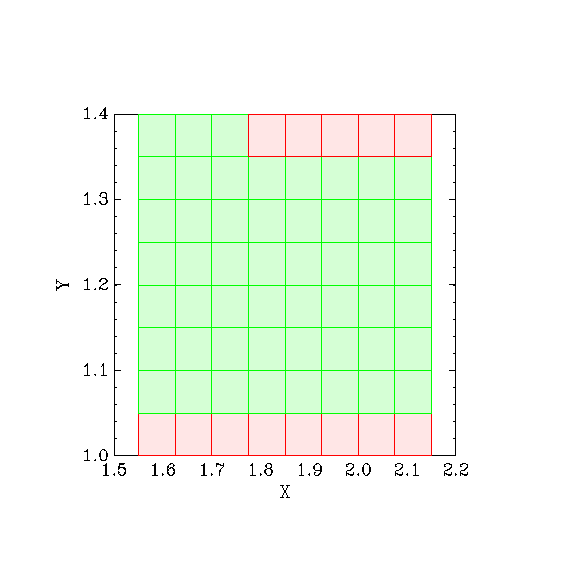
\includegraphics[width=0.6\linewidth,clip,trim=0cm 2.5cm 0cm 2.5cm]{boostdecomposition.png}
 \caption{Controlled region of $R$ using the Euler method for the DC-DC converter.}
 \label{fig:boost_dec}
\end{figure}

We observe on the examples that the resulting control strategies 
synthesized by our method are quite different from those obtained
by the Runge-Kutta method of \cite{NL_minimator} 
(which uses in particular rectangular tiles instead of balls). 
This may explain why the experimental results are here contrasted:
Euler's method works better on 3 examples and worse on the 2 others.
Besides the Euler method fails on one example (DC-DC converter) while {\em DynIBEX} succeeds 
on all of them. Note however that our Euler-based implementation is made
of a few hundreds lines of interpreted code Octave while {\em DynIBEX} is 
made of around five thousands of compiled code C++.

% Our method presents the advantage over the work of \cite{NL_minimator} that
% no numerical integration is required for the control synthesis. 
% 



\subsection{Final Remarks}\label{sec:fr}
We have given a new Euler-based method for controlling sampled switched systems,
and compared it with the Runge-Kutta method of \cite{NL_minimator}. 
The method is remarkably simple and gives already promising results. 
In future work, we plan to explore
the use of the {\em backward} Euler method instead of the forward Euler method used here
(cf: \cite{Beyn2010}).
We plan also to give general sufficient conditions ensuring the convexity
of the error function $\delta_j(\cdot)$; this would allow us to get rid of
the convexity tests that we perform so far numerically for each pattern.






